% **************************************************************************************************************
% A Classic Thesis Style
% An Homage to The Elements of Typographic Style
%
% Copyright (C) 2012 Andr\'e Miede http://www.miede.de
%
% If you like the style then I would appreciate a postcard. My address 
% can be found in the file ClassicThesis.pdf. A collection of the 
% postcards I received so far is available online at 
% http://postcards.miede.de
%
% License:
% This program is free software; you can redistribute it and/or modify
% it under the terms of the GNU General Public License as published by
% the Free Software Foundation; either version 2 of the License, or
% (at your option) any later version.
%
% This program is distributed in the hope that it will be useful,
% but WITHOUT ANY WARRANTY; without even the implied warranty of
% MERCHANTABILITY or FITNESS FOR A PARTICULAR PURPOSE.  See the
% GNU General Public License for more details.
%
% You should have received a copy of the GNU General Public License
% along with this program; see the file COPYING.  If not, write to
% the Free Software Foundation, Inc., 59 Temple Place - Suite 330,
% Boston, MA 02111-1307, USA.
%
% **************************************************************************************************************
% Note:
%    * You must not use "u etc. in strings/commands that will be spaced out (use \"u or real umlauts instead)
%    * New enumeration (small caps): \begin{aenumerate} \end{aenumerate}
%    * For margin notes: \marginpar or \graffito{}
%    * Do not use bold fonts in this style, it is designed around them
%    * Use tables as in the examples
%    * See classicthesis-preamble.sty for useful commands
% **************************************************************************************************************
% To Do:
%		 * [high] Check this out: http://www.golatex.de/koma-script-warnung-in-verbindung-mit-listings-package-t2058.html
%    * [medium] mathbb in section-titles/chapter-titles => disappears somehow in headlines!!!
% **************************************************************************************************************
\documentclass[ twoside,openright,titlepage,numbers=noenddot,headinclude,%1headlines,% letterpaper a4paper
                footinclude=true,cleardoublepage=empty,abstractoff, % <--- obsolete, remove (todo)
                BCOR=5mm,paper=a4,fontsize=11pt,%11pt,a4paper,%
                american,italian,%
                ]{scrreprt}

%********************************************************************
% Note: Make all your adjustments in here
%*******************************************************
% ****************************************************************************************************
% classicthesis-config.tex 
% formerly known as loadpackages.sty, classicthesis-ldpkg.sty, and classicthesis-preamble.sty 
% Use it at the beginning of your ClassicThesis.tex, or as a LaTeX Preamble 
% in your ClassicThesis.{tex,lyx} with % ****************************************************************************************************
% classicthesis-config.tex 
% formerly known as loadpackages.sty, classicthesis-ldpkg.sty, and classicthesis-preamble.sty 
% Use it at the beginning of your ClassicThesis.tex, or as a LaTeX Preamble 
% in your ClassicThesis.{tex,lyx} with % ****************************************************************************************************
% classicthesis-config.tex 
% formerly known as loadpackages.sty, classicthesis-ldpkg.sty, and classicthesis-preamble.sty 
% Use it at the beginning of your ClassicThesis.tex, or as a LaTeX Preamble 
% in your ClassicThesis.{tex,lyx} with \input{classicthesis-config}
% ****************************************************************************************************  
% If you like the classicthesis, then I would appreciate a postcard. 
% My address can be found in the file ClassicThesis.pdf. A collection 
% of the postcards I received so far is available online at 
% http://postcards.miede.de
% ****************************************************************************************************

% ****************************************************************************************************
% 1. Configure classicthesis for your needs here, e.g., remove "drafting" below 
% in order to deactivate the time-stamp on the pages
% ****************************************************************************************************
\PassOptionsToPackage{eulerchapternumbers,listings,drafting,%
				 pdfspacing,%floatperchapter,%linedheaders,%
				 subfig,beramono,eulermath,parts}{classicthesis}										
% ********************************************************************
% Available options for classicthesis.sty 
% (see ClassicThesis.pdf for more information):
% drafting
% parts nochapters linedheaders
% eulerchapternumbers beramono eulermath pdfspacing minionprospacing
% tocaligned dottedtoc manychapters
% listings floatperchapter subfig
% ********************************************************************

% ********************************************************************
% Triggers for this config
% ******************************************************************** 
\usepackage{ifthen}
\newboolean{enable-backrefs} % enable backrefs in the bibliography
\setboolean{enable-backrefs}{false} % true false
% ****************************************************************************************************


% ****************************************************************************************************
% 2. Personal data and user ad-hoc commands
% ****************************************************************************************************
\newcommand{\myTitle}{Sviluppo di prototipi mobile multi-piattaforma con utilizzo di periferiche interne\xspace}
\newcommand{\mySubtitle}{Sottotitolo\xspace}

\newcommand{\myName}{Marco Pezzutti\xspace}
\newcommand{\myProf}{prof.ssa Ombretta Gaggi\xspace}
\newcommand{\myCompany}{Soluzioni Software\xspace}
\newcommand{\myCompanyExtended}{Soluzioni Software S.r.l.\xspace}

\newcommand{\myDegree}{Corso di Laurea in Informatica\xspace}
\newcommand{\myDepartment}{Dipartimento di Matematica\xspace}
\newcommand{\myUni}{Universit\`a degli Studi di Padova\xspace}

\newcommand{\myLocation}{Padova\xspace}
\newcommand{\myTime}{Dicembre 2013\xspace}
\newcommand{\myVersion}{version 0.1\xspace}

\newcommand{\code}[1]{\texttt{#1}\xspace}
% ********************************************************************
% Setup, finetuning, and useful commands
% ********************************************************************
\newcounter{dummy} % necessary for correct hyperlinks (to index, bib, etc.)
\newlength{\abcd} % for ab..z string length calculation
\providecommand{\mLyX}{L\kern-.1667em\lower.25em\hbox{Y}\kern-.125emX\@}
\newcommand{\ie}{i.\,e.}
\newcommand{\Ie}{I.\,e.}
\newcommand{\eg}{e.\,g.}
\newcommand{\Eg}{E.\,g.} 
% ****************************************************************************************************


% ****************************************************************************************************
% 3. Loading some handy packages
% ****************************************************************************************************
% ******************************************************************** 
% Packages with options that might require adjustments
% ******************************************************************** 
\PassOptionsToPackage{utf8}{inputenc}	% latin9 (ISO-8859-9) = latin1+"Euro sign"
 \usepackage{inputenc}				

\PassOptionsToPackage{english,italian}{babel}   % change this to your language(s)
% Spanish languages need extra options in order to work with this template
%\PassOptionsToPackage{spanish,es-lcroman}{babel}
 \usepackage{babel}					

\PassOptionsToPackage{square,numbers}{natbib}
 \usepackage{natbib}				

\PassOptionsToPackage{fleqn}{amsmath}		% math environments and more by the AMS 
 \usepackage{amsmath}

% ******************************************************************** 
% General useful packages
% ******************************************************************** 
\PassOptionsToPackage{T1}{fontenc} % T2A for cyrillics
	\usepackage{fontenc}     
\usepackage{textcomp} % fix warning with missing font shapes
\usepackage{scrhack} % fix warnings when using KOMA with listings package          
\usepackage{xspace} % to get the spacing after macros right  
\usepackage{mparhack} % get marginpar right
\usepackage{fixltx2e} % fixes some LaTeX stuff 
\PassOptionsToPackage{printonlyused,smaller}{acronym}
	\usepackage{acronym} % nice macros for handling all acronyms in the thesis
%\renewcommand*{\acsfont}[1]{\textssc{#1}} % for MinionPro
\renewcommand{\bflabel}[1]{{#1}\hfill} % fix the list of acronyms

\usepackage{amssymb}
% ****************************************************************************************************


% ****************************************************************************************************
% 4. Setup floats: tables, (sub)figures, and captions
% ****************************************************************************************************
\usepackage{tabularx} % better tables
	\setlength{\extrarowheight}{3pt} % increase table row height
\newcommand{\tableheadline}[1]{\multicolumn{1}{c}{\spacedlowsmallcaps{#1}}}
\newcommand{\myfloatalign}{\centering} % to be used with each float for alignment
\usepackage{caption}
\captionsetup{format=hang,font=small}
\usepackage{subfig}
\usepackage{longtable}
\usepackage{multirow}
\PassOptionsToPackage{table}{xcolor}
	\RequirePackage{xcolor}
%\usepackage{colortbl}
\usepackage{threeparttable}
% ****************************************************************************************************


% ****************************************************************************************************
% 5. Setup code listings
% ****************************************************************************************************
\usepackage{listings} 
%\lstset{emph={trueIndex,root},emphstyle=\color{BlueViolet}}%\underbar} % for special keywords
\lstset{language=[LaTeX]Tex,%C++,
    keywordstyle=\color{RoyalBlue},%\bfseries,
    basicstyle=\small\ttfamily,
    %identifierstyle=\color{NavyBlue},
    commentstyle=\color{Green}\ttfamily,
    stringstyle=\rmfamily,
    numbers=none,%left,%
    numberstyle=\scriptsize,%\tiny
    stepnumber=5,
    numbersep=8pt,
    showstringspaces=false,
    breaklines=true,
    frameround=ftff,
    frame=single,
    belowcaptionskip=.75\baselineskip
    %frame=L
} 
% ****************************************************************************************************    		   


% ****************************************************************************************************
% 6. PDFLaTeX, hyperreferences and citation backreferences
% ****************************************************************************************************
% ********************************************************************
% Using PDFLaTeX
% ********************************************************************
\PassOptionsToPackage{pdftex,hyperfootnotes=true,pdfpagelabels}{hyperref}
	\usepackage{hyperref}  % backref linktocpage pagebackref
\pdfcompresslevel=9
\pdfadjustspacing=1 
\PassOptionsToPackage{pdftex}{graphicx}
	\usepackage{graphicx} 

% ********************************************************************
% Setup the style of the backrefs from the bibliography
% (translate the options to any language you use)
% ********************************************************************
\newcommand{\backrefnotcitedstring}{\relax}%(Not cited.)
\newcommand{\backrefcitedsinglestring}[1]{(Cited on page~#1.)}
\newcommand{\backrefcitedmultistring}[1]{(Cited on pages~#1.)}
\ifthenelse{\boolean{enable-backrefs}}%
{%
		\PassOptionsToPackage{hyperpageref}{backref}
		\usepackage{backref} % to be loaded after hyperref package 
		   \renewcommand{\backreftwosep}{ and~} % separate 2 pages
		   \renewcommand{\backreflastsep}{, and~} % separate last of longer list
		   \renewcommand*{\backref}[1]{}  % disable standard
		   \renewcommand*{\backrefalt}[4]{% detailed backref
		      \ifcase #1 %
		         \backrefnotcitedstring%
		      \or%
		         \backrefcitedsinglestring{#2}%
		      \else%
		         \backrefcitedmultistring{#2}%
		      \fi}%
}{\relax}    

% ********************************************************************
% Hyperreferences
% ********************************************************************
\hypersetup{%
    %draft,	% = no hyperlinking at all (useful in b/w printouts)
    colorlinks=true, linktocpage=true, pdfstartpage=3, pdfstartview=FitV,%
    % uncomment the following line if you want to have black links (e.g., for printing)
    %colorlinks=false, linktocpage=false, pdfborder={0 0 0}, pdfstartpage=3, pdfstartview=FitV,% 
    breaklinks=true, pdfpagemode=UseNone, pageanchor=true, pdfpagemode=UseOutlines,%
    plainpages=false, bookmarksnumbered, bookmarksopen=true, bookmarksopenlevel=1,%
    hypertexnames=true, pdfhighlight=/O,%nesting=true,%frenchlinks,%
    urlcolor=webbrown, linkcolor=RoyalBlue, citecolor=webgreen, %pagecolor=RoyalBlue,%
    %urlcolor=Black, linkcolor=Black, citecolor=Black, %pagecolor=Black,%
    pdftitle={\myTitle},%
    pdfauthor={\textcopyright\ \myName, \myUni, \myDegree},%
    pdfsubject={},%
    pdfkeywords={},%
    pdfcreator={pdfLaTeX},%
    pdfproducer={LaTeX with hyperref and classicthesis}%
}   

% ********************************************************************
% Setup autoreferences
% ********************************************************************
% There are some issues regarding autorefnames
% http://www.ureader.de/msg/136221647.aspx
% http://www.tex.ac.uk/cgi-bin/texfaq2html?label=latexwords
% you have to redefine the makros for the 
% language you use, e.g., american, ngerman
% (as chosen when loading babel/AtBeginDocument)
% ********************************************************************
\makeatletter
\@ifpackageloaded{babel}%
    {%
       \addto\extrasamerican{%
					\renewcommand*{\figureautorefname}{Figure}%
					\renewcommand*{\tableautorefname}{Table}%
					\renewcommand*{\partautorefname}{Part}%
					\renewcommand*{\chapterautorefname}{Chapter}%
					\renewcommand*{\sectionautorefname}{Section}%
					\renewcommand*{\subsectionautorefname}{Section}%
					\renewcommand*{\subsubsectionautorefname}{Section}% 	
				}%
       \addto\extrasngerman{% 
					\renewcommand*{\paragraphautorefname}{Absatz}%
					\renewcommand*{\subparagraphautorefname}{Unterabsatz}%
					\renewcommand*{\footnoteautorefname}{Fu\"snote}%
					\renewcommand*{\FancyVerbLineautorefname}{Zeile}%
					\renewcommand*{\theoremautorefname}{Theorem}%
					\renewcommand*{\appendixautorefname}{Anhang}%
					\renewcommand*{\equationautorefname}{Gleichung}%        
					\renewcommand*{\itemautorefname}{Punkt}%
				}%	
			% Fix to getting autorefs for subfigures right (thanks to Belinda Vogt for changing the definition)
			\providecommand{\subfigureautorefname}{\figureautorefname}%  			
    }{\relax}
\makeatother


% ****************************************************************************************************
% 7. Last calls before the bar closes
% ****************************************************************************************************
% ********************************************************************
% Development Stuff
% ********************************************************************
\listfiles
%\PassOptionsToPackage{l2tabu,orthodox,abort}{nag}
%	\usepackage{nag}
%\PassOptionsToPackage{warning, all}{onlyamsmath}
%	\usepackage{onlyamsmath}

% ********************************************************************
% Last, but not least...
% ********************************************************************
\usepackage{classicthesis} 
% ****************************************************************************************************


% ****************************************************************************************************
% 8. Further adjustments (experimental)
% ****************************************************************************************************
% ********************************************************************
% Changing the text area
% ********************************************************************
%\linespread{1.05} % a bit more for Palatino
%\areaset[current]{312pt}{761pt} % 686 (factor 2.2) + 33 head + 42 head \the\footskip
%\setlength{\marginparwidth}{7em}%
%\setlength{\marginparsep}{2em}%

% ********************************************************************
% Using different fonts
% ********************************************************************
%\usepackage[oldstylenums]{kpfonts} % oldstyle notextcomp
%\usepackage[osf]{libertine}
%\usepackage{hfoldsty} % Computer Modern with osf
%\usepackage[light,condensed,math]{iwona}
%\renewcommand{\sfdefault}{iwona}
%\usepackage{lmodern} % <-- no osf support :-(
%\usepackage[urw-garamond]{mathdesign} <-- no osf support :-(
% ****************************************************************************************************

% ****************************************************************************************************  
% If you like the classicthesis, then I would appreciate a postcard. 
% My address can be found in the file ClassicThesis.pdf. A collection 
% of the postcards I received so far is available online at 
% http://postcards.miede.de
% ****************************************************************************************************

% ****************************************************************************************************
% 1. Configure classicthesis for your needs here, e.g., remove "drafting" below 
% in order to deactivate the time-stamp on the pages
% ****************************************************************************************************
\PassOptionsToPackage{eulerchapternumbers,listings,drafting,%
				 pdfspacing,%floatperchapter,%linedheaders,%
				 subfig,beramono,eulermath,parts}{classicthesis}										
% ********************************************************************
% Available options for classicthesis.sty 
% (see ClassicThesis.pdf for more information):
% drafting
% parts nochapters linedheaders
% eulerchapternumbers beramono eulermath pdfspacing minionprospacing
% tocaligned dottedtoc manychapters
% listings floatperchapter subfig
% ********************************************************************

% ********************************************************************
% Triggers for this config
% ******************************************************************** 
\usepackage{ifthen}
\newboolean{enable-backrefs} % enable backrefs in the bibliography
\setboolean{enable-backrefs}{false} % true false
% ****************************************************************************************************


% ****************************************************************************************************
% 2. Personal data and user ad-hoc commands
% ****************************************************************************************************
\newcommand{\myTitle}{Sviluppo di prototipi mobile multi-piattaforma con utilizzo di periferiche interne\xspace}
\newcommand{\mySubtitle}{Sottotitolo\xspace}

\newcommand{\myName}{Marco Pezzutti\xspace}
\newcommand{\myProf}{prof.ssa Ombretta Gaggi\xspace}
\newcommand{\myCompany}{Soluzioni Software\xspace}
\newcommand{\myCompanyExtended}{Soluzioni Software S.r.l.\xspace}

\newcommand{\myDegree}{Corso di Laurea in Informatica\xspace}
\newcommand{\myDepartment}{Dipartimento di Matematica\xspace}
\newcommand{\myUni}{Universit\`a degli Studi di Padova\xspace}

\newcommand{\myLocation}{Padova\xspace}
\newcommand{\myTime}{Dicembre 2013\xspace}
\newcommand{\myVersion}{version 0.1\xspace}

\newcommand{\code}[1]{\texttt{#1}\xspace}
% ********************************************************************
% Setup, finetuning, and useful commands
% ********************************************************************
\newcounter{dummy} % necessary for correct hyperlinks (to index, bib, etc.)
\newlength{\abcd} % for ab..z string length calculation
\providecommand{\mLyX}{L\kern-.1667em\lower.25em\hbox{Y}\kern-.125emX\@}
\newcommand{\ie}{i.\,e.}
\newcommand{\Ie}{I.\,e.}
\newcommand{\eg}{e.\,g.}
\newcommand{\Eg}{E.\,g.} 
% ****************************************************************************************************


% ****************************************************************************************************
% 3. Loading some handy packages
% ****************************************************************************************************
% ******************************************************************** 
% Packages with options that might require adjustments
% ******************************************************************** 
\PassOptionsToPackage{utf8}{inputenc}	% latin9 (ISO-8859-9) = latin1+"Euro sign"
 \usepackage{inputenc}				

\PassOptionsToPackage{english,italian}{babel}   % change this to your language(s)
% Spanish languages need extra options in order to work with this template
%\PassOptionsToPackage{spanish,es-lcroman}{babel}
 \usepackage{babel}					

\PassOptionsToPackage{square,numbers}{natbib}
 \usepackage{natbib}				

\PassOptionsToPackage{fleqn}{amsmath}		% math environments and more by the AMS 
 \usepackage{amsmath}

% ******************************************************************** 
% General useful packages
% ******************************************************************** 
\PassOptionsToPackage{T1}{fontenc} % T2A for cyrillics
	\usepackage{fontenc}     
\usepackage{textcomp} % fix warning with missing font shapes
\usepackage{scrhack} % fix warnings when using KOMA with listings package          
\usepackage{xspace} % to get the spacing after macros right  
\usepackage{mparhack} % get marginpar right
\usepackage{fixltx2e} % fixes some LaTeX stuff 
\PassOptionsToPackage{printonlyused,smaller}{acronym}
	\usepackage{acronym} % nice macros for handling all acronyms in the thesis
%\renewcommand*{\acsfont}[1]{\textssc{#1}} % for MinionPro
\renewcommand{\bflabel}[1]{{#1}\hfill} % fix the list of acronyms

\usepackage{amssymb}
% ****************************************************************************************************


% ****************************************************************************************************
% 4. Setup floats: tables, (sub)figures, and captions
% ****************************************************************************************************
\usepackage{tabularx} % better tables
	\setlength{\extrarowheight}{3pt} % increase table row height
\newcommand{\tableheadline}[1]{\multicolumn{1}{c}{\spacedlowsmallcaps{#1}}}
\newcommand{\myfloatalign}{\centering} % to be used with each float for alignment
\usepackage{caption}
\captionsetup{format=hang,font=small}
\usepackage{subfig}
\usepackage{longtable}
\usepackage{multirow}
\PassOptionsToPackage{table}{xcolor}
	\RequirePackage{xcolor}
%\usepackage{colortbl}
\usepackage{threeparttable}
% ****************************************************************************************************


% ****************************************************************************************************
% 5. Setup code listings
% ****************************************************************************************************
\usepackage{listings} 
%\lstset{emph={trueIndex,root},emphstyle=\color{BlueViolet}}%\underbar} % for special keywords
\lstset{language=[LaTeX]Tex,%C++,
    keywordstyle=\color{RoyalBlue},%\bfseries,
    basicstyle=\small\ttfamily,
    %identifierstyle=\color{NavyBlue},
    commentstyle=\color{Green}\ttfamily,
    stringstyle=\rmfamily,
    numbers=none,%left,%
    numberstyle=\scriptsize,%\tiny
    stepnumber=5,
    numbersep=8pt,
    showstringspaces=false,
    breaklines=true,
    frameround=ftff,
    frame=single,
    belowcaptionskip=.75\baselineskip
    %frame=L
} 
% ****************************************************************************************************    		   


% ****************************************************************************************************
% 6. PDFLaTeX, hyperreferences and citation backreferences
% ****************************************************************************************************
% ********************************************************************
% Using PDFLaTeX
% ********************************************************************
\PassOptionsToPackage{pdftex,hyperfootnotes=true,pdfpagelabels}{hyperref}
	\usepackage{hyperref}  % backref linktocpage pagebackref
\pdfcompresslevel=9
\pdfadjustspacing=1 
\PassOptionsToPackage{pdftex}{graphicx}
	\usepackage{graphicx} 

% ********************************************************************
% Setup the style of the backrefs from the bibliography
% (translate the options to any language you use)
% ********************************************************************
\newcommand{\backrefnotcitedstring}{\relax}%(Not cited.)
\newcommand{\backrefcitedsinglestring}[1]{(Cited on page~#1.)}
\newcommand{\backrefcitedmultistring}[1]{(Cited on pages~#1.)}
\ifthenelse{\boolean{enable-backrefs}}%
{%
		\PassOptionsToPackage{hyperpageref}{backref}
		\usepackage{backref} % to be loaded after hyperref package 
		   \renewcommand{\backreftwosep}{ and~} % separate 2 pages
		   \renewcommand{\backreflastsep}{, and~} % separate last of longer list
		   \renewcommand*{\backref}[1]{}  % disable standard
		   \renewcommand*{\backrefalt}[4]{% detailed backref
		      \ifcase #1 %
		         \backrefnotcitedstring%
		      \or%
		         \backrefcitedsinglestring{#2}%
		      \else%
		         \backrefcitedmultistring{#2}%
		      \fi}%
}{\relax}    

% ********************************************************************
% Hyperreferences
% ********************************************************************
\hypersetup{%
    %draft,	% = no hyperlinking at all (useful in b/w printouts)
    colorlinks=true, linktocpage=true, pdfstartpage=3, pdfstartview=FitV,%
    % uncomment the following line if you want to have black links (e.g., for printing)
    %colorlinks=false, linktocpage=false, pdfborder={0 0 0}, pdfstartpage=3, pdfstartview=FitV,% 
    breaklinks=true, pdfpagemode=UseNone, pageanchor=true, pdfpagemode=UseOutlines,%
    plainpages=false, bookmarksnumbered, bookmarksopen=true, bookmarksopenlevel=1,%
    hypertexnames=true, pdfhighlight=/O,%nesting=true,%frenchlinks,%
    urlcolor=webbrown, linkcolor=RoyalBlue, citecolor=webgreen, %pagecolor=RoyalBlue,%
    %urlcolor=Black, linkcolor=Black, citecolor=Black, %pagecolor=Black,%
    pdftitle={\myTitle},%
    pdfauthor={\textcopyright\ \myName, \myUni, \myDegree},%
    pdfsubject={},%
    pdfkeywords={},%
    pdfcreator={pdfLaTeX},%
    pdfproducer={LaTeX with hyperref and classicthesis}%
}   

% ********************************************************************
% Setup autoreferences
% ********************************************************************
% There are some issues regarding autorefnames
% http://www.ureader.de/msg/136221647.aspx
% http://www.tex.ac.uk/cgi-bin/texfaq2html?label=latexwords
% you have to redefine the makros for the 
% language you use, e.g., american, ngerman
% (as chosen when loading babel/AtBeginDocument)
% ********************************************************************
\makeatletter
\@ifpackageloaded{babel}%
    {%
       \addto\extrasamerican{%
					\renewcommand*{\figureautorefname}{Figure}%
					\renewcommand*{\tableautorefname}{Table}%
					\renewcommand*{\partautorefname}{Part}%
					\renewcommand*{\chapterautorefname}{Chapter}%
					\renewcommand*{\sectionautorefname}{Section}%
					\renewcommand*{\subsectionautorefname}{Section}%
					\renewcommand*{\subsubsectionautorefname}{Section}% 	
				}%
       \addto\extrasngerman{% 
					\renewcommand*{\paragraphautorefname}{Absatz}%
					\renewcommand*{\subparagraphautorefname}{Unterabsatz}%
					\renewcommand*{\footnoteautorefname}{Fu\"snote}%
					\renewcommand*{\FancyVerbLineautorefname}{Zeile}%
					\renewcommand*{\theoremautorefname}{Theorem}%
					\renewcommand*{\appendixautorefname}{Anhang}%
					\renewcommand*{\equationautorefname}{Gleichung}%        
					\renewcommand*{\itemautorefname}{Punkt}%
				}%	
			% Fix to getting autorefs for subfigures right (thanks to Belinda Vogt for changing the definition)
			\providecommand{\subfigureautorefname}{\figureautorefname}%  			
    }{\relax}
\makeatother


% ****************************************************************************************************
% 7. Last calls before the bar closes
% ****************************************************************************************************
% ********************************************************************
% Development Stuff
% ********************************************************************
\listfiles
%\PassOptionsToPackage{l2tabu,orthodox,abort}{nag}
%	\usepackage{nag}
%\PassOptionsToPackage{warning, all}{onlyamsmath}
%	\usepackage{onlyamsmath}

% ********************************************************************
% Last, but not least...
% ********************************************************************
\usepackage{classicthesis} 
% ****************************************************************************************************


% ****************************************************************************************************
% 8. Further adjustments (experimental)
% ****************************************************************************************************
% ********************************************************************
% Changing the text area
% ********************************************************************
%\linespread{1.05} % a bit more for Palatino
%\areaset[current]{312pt}{761pt} % 686 (factor 2.2) + 33 head + 42 head \the\footskip
%\setlength{\marginparwidth}{7em}%
%\setlength{\marginparsep}{2em}%

% ********************************************************************
% Using different fonts
% ********************************************************************
%\usepackage[oldstylenums]{kpfonts} % oldstyle notextcomp
%\usepackage[osf]{libertine}
%\usepackage{hfoldsty} % Computer Modern with osf
%\usepackage[light,condensed,math]{iwona}
%\renewcommand{\sfdefault}{iwona}
%\usepackage{lmodern} % <-- no osf support :-(
%\usepackage[urw-garamond]{mathdesign} <-- no osf support :-(
% ****************************************************************************************************

% ****************************************************************************************************  
% If you like the classicthesis, then I would appreciate a postcard. 
% My address can be found in the file ClassicThesis.pdf. A collection 
% of the postcards I received so far is available online at 
% http://postcards.miede.de
% ****************************************************************************************************

% ****************************************************************************************************
% 1. Configure classicthesis for your needs here, e.g., remove "drafting" below 
% in order to deactivate the time-stamp on the pages
% ****************************************************************************************************
\PassOptionsToPackage{eulerchapternumbers,listings,drafting,%
				 pdfspacing,%floatperchapter,%linedheaders,%
				 subfig,beramono,eulermath,parts}{classicthesis}										
% ********************************************************************
% Available options for classicthesis.sty 
% (see ClassicThesis.pdf for more information):
% drafting
% parts nochapters linedheaders
% eulerchapternumbers beramono eulermath pdfspacing minionprospacing
% tocaligned dottedtoc manychapters
% listings floatperchapter subfig
% ********************************************************************

% ********************************************************************
% Triggers for this config
% ******************************************************************** 
\usepackage{ifthen}
\newboolean{enable-backrefs} % enable backrefs in the bibliography
\setboolean{enable-backrefs}{false} % true false
% ****************************************************************************************************


% ****************************************************************************************************
% 2. Personal data and user ad-hoc commands
% ****************************************************************************************************
\newcommand{\myTitle}{Sviluppo di prototipi mobile multi-piattaforma con utilizzo di periferiche interne\xspace}
\newcommand{\mySubtitle}{Sottotitolo\xspace}

\newcommand{\myName}{Marco Pezzutti\xspace}
\newcommand{\myProf}{prof.ssa Ombretta Gaggi\xspace}
\newcommand{\myCompany}{Soluzioni Software\xspace}
\newcommand{\myCompanyExtended}{Soluzioni Software S.r.l.\xspace}

\newcommand{\myDegree}{Corso di Laurea in Informatica\xspace}
\newcommand{\myDepartment}{Dipartimento di Matematica\xspace}
\newcommand{\myUni}{Universit\`a degli Studi di Padova\xspace}

\newcommand{\myLocation}{Padova\xspace}
\newcommand{\myTime}{Dicembre 2013\xspace}
\newcommand{\myVersion}{version 0.1\xspace}

\newcommand{\code}[1]{\texttt{#1}\xspace}
% ********************************************************************
% Setup, finetuning, and useful commands
% ********************************************************************
\newcounter{dummy} % necessary for correct hyperlinks (to index, bib, etc.)
\newlength{\abcd} % for ab..z string length calculation
\providecommand{\mLyX}{L\kern-.1667em\lower.25em\hbox{Y}\kern-.125emX\@}
\newcommand{\ie}{i.\,e.}
\newcommand{\Ie}{I.\,e.}
\newcommand{\eg}{e.\,g.}
\newcommand{\Eg}{E.\,g.} 
% ****************************************************************************************************


% ****************************************************************************************************
% 3. Loading some handy packages
% ****************************************************************************************************
% ******************************************************************** 
% Packages with options that might require adjustments
% ******************************************************************** 
\PassOptionsToPackage{utf8}{inputenc}	% latin9 (ISO-8859-9) = latin1+"Euro sign"
 \usepackage{inputenc}				

\PassOptionsToPackage{english,italian}{babel}   % change this to your language(s)
% Spanish languages need extra options in order to work with this template
%\PassOptionsToPackage{spanish,es-lcroman}{babel}
 \usepackage{babel}					

\PassOptionsToPackage{square,numbers}{natbib}
 \usepackage{natbib}				

\PassOptionsToPackage{fleqn}{amsmath}		% math environments and more by the AMS 
 \usepackage{amsmath}

% ******************************************************************** 
% General useful packages
% ******************************************************************** 
\PassOptionsToPackage{T1}{fontenc} % T2A for cyrillics
	\usepackage{fontenc}     
\usepackage{textcomp} % fix warning with missing font shapes
\usepackage{scrhack} % fix warnings when using KOMA with listings package          
\usepackage{xspace} % to get the spacing after macros right  
\usepackage{mparhack} % get marginpar right
\usepackage{fixltx2e} % fixes some LaTeX stuff 
\PassOptionsToPackage{printonlyused,smaller}{acronym}
	\usepackage{acronym} % nice macros for handling all acronyms in the thesis
%\renewcommand*{\acsfont}[1]{\textssc{#1}} % for MinionPro
\renewcommand{\bflabel}[1]{{#1}\hfill} % fix the list of acronyms

\usepackage{amssymb}
% ****************************************************************************************************


% ****************************************************************************************************
% 4. Setup floats: tables, (sub)figures, and captions
% ****************************************************************************************************
\usepackage{tabularx} % better tables
	\setlength{\extrarowheight}{3pt} % increase table row height
\newcommand{\tableheadline}[1]{\multicolumn{1}{c}{\spacedlowsmallcaps{#1}}}
\newcommand{\myfloatalign}{\centering} % to be used with each float for alignment
\usepackage{caption}
\captionsetup{format=hang,font=small}
\usepackage{subfig}
\usepackage{longtable}
\usepackage{multirow}
\PassOptionsToPackage{table}{xcolor}
	\RequirePackage{xcolor}
%\usepackage{colortbl}
\usepackage{threeparttable}
% ****************************************************************************************************


% ****************************************************************************************************
% 5. Setup code listings
% ****************************************************************************************************
\usepackage{listings} 
%\lstset{emph={trueIndex,root},emphstyle=\color{BlueViolet}}%\underbar} % for special keywords
\lstset{language=[LaTeX]Tex,%C++,
    keywordstyle=\color{RoyalBlue},%\bfseries,
    basicstyle=\small\ttfamily,
    %identifierstyle=\color{NavyBlue},
    commentstyle=\color{Green}\ttfamily,
    stringstyle=\rmfamily,
    numbers=none,%left,%
    numberstyle=\scriptsize,%\tiny
    stepnumber=5,
    numbersep=8pt,
    showstringspaces=false,
    breaklines=true,
    frameround=ftff,
    frame=single,
    belowcaptionskip=.75\baselineskip
    %frame=L
} 
% ****************************************************************************************************    		   


% ****************************************************************************************************
% 6. PDFLaTeX, hyperreferences and citation backreferences
% ****************************************************************************************************
% ********************************************************************
% Using PDFLaTeX
% ********************************************************************
\PassOptionsToPackage{pdftex,hyperfootnotes=true,pdfpagelabels}{hyperref}
	\usepackage{hyperref}  % backref linktocpage pagebackref
\pdfcompresslevel=9
\pdfadjustspacing=1 
\PassOptionsToPackage{pdftex}{graphicx}
	\usepackage{graphicx} 

% ********************************************************************
% Setup the style of the backrefs from the bibliography
% (translate the options to any language you use)
% ********************************************************************
\newcommand{\backrefnotcitedstring}{\relax}%(Not cited.)
\newcommand{\backrefcitedsinglestring}[1]{(Cited on page~#1.)}
\newcommand{\backrefcitedmultistring}[1]{(Cited on pages~#1.)}
\ifthenelse{\boolean{enable-backrefs}}%
{%
		\PassOptionsToPackage{hyperpageref}{backref}
		\usepackage{backref} % to be loaded after hyperref package 
		   \renewcommand{\backreftwosep}{ and~} % separate 2 pages
		   \renewcommand{\backreflastsep}{, and~} % separate last of longer list
		   \renewcommand*{\backref}[1]{}  % disable standard
		   \renewcommand*{\backrefalt}[4]{% detailed backref
		      \ifcase #1 %
		         \backrefnotcitedstring%
		      \or%
		         \backrefcitedsinglestring{#2}%
		      \else%
		         \backrefcitedmultistring{#2}%
		      \fi}%
}{\relax}    

% ********************************************************************
% Hyperreferences
% ********************************************************************
\hypersetup{%
    %draft,	% = no hyperlinking at all (useful in b/w printouts)
    colorlinks=true, linktocpage=true, pdfstartpage=3, pdfstartview=FitV,%
    % uncomment the following line if you want to have black links (e.g., for printing)
    %colorlinks=false, linktocpage=false, pdfborder={0 0 0}, pdfstartpage=3, pdfstartview=FitV,% 
    breaklinks=true, pdfpagemode=UseNone, pageanchor=true, pdfpagemode=UseOutlines,%
    plainpages=false, bookmarksnumbered, bookmarksopen=true, bookmarksopenlevel=1,%
    hypertexnames=true, pdfhighlight=/O,%nesting=true,%frenchlinks,%
    urlcolor=webbrown, linkcolor=RoyalBlue, citecolor=webgreen, %pagecolor=RoyalBlue,%
    %urlcolor=Black, linkcolor=Black, citecolor=Black, %pagecolor=Black,%
    pdftitle={\myTitle},%
    pdfauthor={\textcopyright\ \myName, \myUni, \myDegree},%
    pdfsubject={},%
    pdfkeywords={},%
    pdfcreator={pdfLaTeX},%
    pdfproducer={LaTeX with hyperref and classicthesis}%
}   

% ********************************************************************
% Setup autoreferences
% ********************************************************************
% There are some issues regarding autorefnames
% http://www.ureader.de/msg/136221647.aspx
% http://www.tex.ac.uk/cgi-bin/texfaq2html?label=latexwords
% you have to redefine the makros for the 
% language you use, e.g., american, ngerman
% (as chosen when loading babel/AtBeginDocument)
% ********************************************************************
\makeatletter
\@ifpackageloaded{babel}%
    {%
       \addto\extrasamerican{%
					\renewcommand*{\figureautorefname}{Figure}%
					\renewcommand*{\tableautorefname}{Table}%
					\renewcommand*{\partautorefname}{Part}%
					\renewcommand*{\chapterautorefname}{Chapter}%
					\renewcommand*{\sectionautorefname}{Section}%
					\renewcommand*{\subsectionautorefname}{Section}%
					\renewcommand*{\subsubsectionautorefname}{Section}% 	
				}%
       \addto\extrasngerman{% 
					\renewcommand*{\paragraphautorefname}{Absatz}%
					\renewcommand*{\subparagraphautorefname}{Unterabsatz}%
					\renewcommand*{\footnoteautorefname}{Fu\"snote}%
					\renewcommand*{\FancyVerbLineautorefname}{Zeile}%
					\renewcommand*{\theoremautorefname}{Theorem}%
					\renewcommand*{\appendixautorefname}{Anhang}%
					\renewcommand*{\equationautorefname}{Gleichung}%        
					\renewcommand*{\itemautorefname}{Punkt}%
				}%	
			% Fix to getting autorefs for subfigures right (thanks to Belinda Vogt for changing the definition)
			\providecommand{\subfigureautorefname}{\figureautorefname}%  			
    }{\relax}
\makeatother


% ****************************************************************************************************
% 7. Last calls before the bar closes
% ****************************************************************************************************
% ********************************************************************
% Development Stuff
% ********************************************************************
\listfiles
%\PassOptionsToPackage{l2tabu,orthodox,abort}{nag}
%	\usepackage{nag}
%\PassOptionsToPackage{warning, all}{onlyamsmath}
%	\usepackage{onlyamsmath}

% ********************************************************************
% Last, but not least...
% ********************************************************************
\usepackage{classicthesis} 
% ****************************************************************************************************


% ****************************************************************************************************
% 8. Further adjustments (experimental)
% ****************************************************************************************************
% ********************************************************************
% Changing the text area
% ********************************************************************
%\linespread{1.05} % a bit more for Palatino
%\areaset[current]{312pt}{761pt} % 686 (factor 2.2) + 33 head + 42 head \the\footskip
%\setlength{\marginparwidth}{7em}%
%\setlength{\marginparsep}{2em}%

% ********************************************************************
% Using different fonts
% ********************************************************************
%\usepackage[oldstylenums]{kpfonts} % oldstyle notextcomp
%\usepackage[osf]{libertine}
%\usepackage{hfoldsty} % Computer Modern with osf
%\usepackage[light,condensed,math]{iwona}
%\renewcommand{\sfdefault}{iwona}
%\usepackage{lmodern} % <-- no osf support :-(
%\usepackage[urw-garamond]{mathdesign} <-- no osf support :-(
% ****************************************************************************************************


%********************************************************************
% Hyphenation
%*******************************************************
%\hyphenation{multi-linguaggio}

% ********************************************************************
% GO!GO!GO! MOVE IT!
%*******************************************************
\begin{document}
\frenchspacing
\raggedbottom
\selectlanguage{italian} % american italian
%\renewcommand*{\bibname}{new name}
%\setbibpreamble{}
\pagenumbering{roman}
\pagestyle{plain}
%********************************************************************
% Frontmatter
%*******************************************************
%%*******************************************************
% Little Dirty Titlepage
%*******************************************************
\thispagestyle{empty}
%\pdfbookmark[1]{Titel}{title}
%*******************************************************
\begin{center}
    \spacedlowsmallcaps{\myName} \\ \medskip                        

    \begingroup
        \color{Maroon}\spacedallcaps{\myTitle}
    \endgroup
\end{center}        

%*******************************************************
% Titlepage
%*******************************************************
\begin{titlepage}
	% if you want the titlepage to be centered, uncomment and fine-tune the line below (KOMA classes environment)
	\begin{addmargin}[-1cm]{-3cm}
    \begin{center}
        \large  

        \hfill

        \vfill

        \begingroup
        	\textcolor{redUni}{\textls[160]{\scshape{\huge \myUni}}}\\ \bigskip
        	
        	\textls[80]{\scshape{\huge \myDepartment}}\\ \medskip
        	
			\textls[80]{\scshape{\LARGE \myDegree}}\\
            
        \endgroup

        \vfill

        
\includegraphics[width=5cm]{gfx/unipd_sigillo} \\ \medskip
		
		\vfill		
		
		\textcolor{redUni}{\textls[80]{\scshape{\huge \myTitle}}} \\ \medskip
        %\mySubtitle \\
        
        \vfill
        
        
		\begin{minipage}{0.5\textwidth}
			\begin{flushleft}
			\emph{Laureando:}\\
			\textsc{\Large \myName}
			\end{flushleft}
		\end{minipage}
		\begin{minipage}{0.5\textwidth}
			\begin{flushright}
			\emph{Relatore:}\\
			\textsc{\Large \myProf}
			\end{flushright}
		\end{minipage}        
        
		\vfill

        \myTime
                    

    \end{center}  
  \end{addmargin}       
\end{titlepage}   
%\thispagestyle{empty}

\hfill

\vfill

\noindent\myName: \textit{\myTitle,} \mySubtitle, %\myDegree, 
\textcopyright\ \myTime

%\bigskip
%
%\noindent\spacedlowsmallcaps{Supervisors}: \\
%\myProf \\
%\myOtherProf \\ 
%\mySupervisor
%
%\medskip
%
%\noindent\spacedlowsmallcaps{Location}: \\
%\myLocation
%
%\medskip
%
%\noindent\spacedlowsmallcaps{Time Frame}: \\
%\myTime

\cleardoublepage%*******************************************************
% Dedication
%*******************************************************
\thispagestyle{empty}
%\phantomsection 
\refstepcounter{dummy}
\pdfbookmark[1]{Dedica}{Dedica}

\vspace*{3cm}

\begin{center}
    \LARGE{A Greta}
\end{center}

\medskip

\begin{center}
    \LARGE{A mamma e papà}
\end{center}
%\cleardoublepage\include{FrontBackmatter/Foreword}
\cleardoublepage%*******************************************************
% Abstract
%*******************************************************
%\renewcommand{\abstractname}{Abstract}
\pdfbookmark[1]{Abstract}{Abstract}
\begingroup
\let\clearpage\relax
\let\cleardoublepage\relax
\let\cleardoublepage\relax

\chapter*{Abstract}
Tale documento rappresenta la tesi di laurea triennale del laureando \myName e si prefigge di descrivere tutte le attività inerenti lo stage, svolto presso la ditta \myCompany , riguardante lo sviluppo di un'applicazione multi-piattaforma utilizzando il framework Sencha Touch 2 e la piattaforma Apache Cordova.

Lo sviluppo dell'applicazione è uno studio su tali tecnologie e su come esse possano essere utilizzate efficacemente per interagire con i sensori interni ai device mobili quali GPS, fotocamera e microfono con lo scopo di acquisire informazioni utili al business aziendale.

Il prodotto di questo studio è una serie di applicazioni per sistemi mobili quali Android e iOS che avranno lo scopo di illustrare tutte le funzionalità che è stato possibile implementare e da cui la stessa azienda potrà prendere spunto per sviluppare le sue prossime applicazioni.



\endgroup

\vfill
%\cleardoublepage%*******************************************************
% Publications
%*******************************************************
\pdfbookmark[1]{Publications}{publications}
\chapter*{Publications}
Some ideas and figures have appeared previously in the following publications:

\bigskip

\noindent Put your publications from the thesis here. The packages \texttt{multibib} or \texttt{bibtopic} etc. can be used to handle multiple different bibliographies in your document.
\cleardoublepage%*******************************************************
% Acknowledgments
%*******************************************************
\pdfbookmark[1]{Ringraziamenti}{Ringraziamenti}

\bigskip

\begingroup
\let\clearpage\relax
\let\cleardoublepage\relax
\let\cleardoublepage\relax
\chapter*{Ringraziamenti}
Innanzitutto desidero ringraziare la mia relatrice, professoressa Ombretta Gaggi, per il tempo che mi ha dedicato e per aver contribuito al completamento di questa tesi con i suoi preziosi consigli.\\

Ringrazio l'azienda \myCompany per avermi permesso di svolgere un progetto interessante e attuale e per avermi accolto in un ambiente sereno ma allo stesso tempo serio e professionale.
Ringrazio il mio tutor Santo Bruno, che mi ha guidato nei momenti critici e ringrazio tutto lo staff che ha saputo donarmi sorrisi e buoni suggerimenti in ogni momento della giornata lavorativa.\\

Ringrazio tutti gli amici che mi hanno supportato e sopportato in questi lunghi anni, che hanno saputo gioire con me dei risultati ottenuti e mi hanno sostenuto nei momenti difficili.\\

Ringrazio con tutto il cuore Greta, senza di lei non avrei mai raggiunto questo traguardo; con la sua forza di volontà mi ha saputo spronare e motivare in ogni istante e mi ha fatto apprezzare la gioia e la soddisfazione di ogni ostacolo superato. La ringrazio di aver creduto in me più di chiunque altro e di avermi dato la forza per compiere questo percorso.\\

Infine voglio ringraziare tutta la mia famiglia, ma soprattutto mamma e papà che, nonostante i fallimenti passati, hanno saputo credere in me e darmi fiducia per affrontare questo impegnativo cammino con la testa alta e senza paura di sbagliare.

\vspace{2cm}

\begin{center}
\emph{Grazie a tutti, di cuore}
\end{center}

\endgroup




\pagestyle{scrheadings}
\cleardoublepage%*******************************************************
% Table of Contents
%*******************************************************
%\phantomsection
\refstepcounter{dummy}
\pdfbookmark[1]{\contentsname}{tableofcontents}
\setcounter{tocdepth}{2} % <-- 2 includes up to subsections in the ToC
\setcounter{secnumdepth}{3} % <-- 3 numbers up to subsubsections
\manualmark
\markboth{\spacedlowsmallcaps{\contentsname}}{\spacedlowsmallcaps{\contentsname}}
\tableofcontents 
\automark[section]{chapter}
\renewcommand{\chaptermark}[1]{\markboth{\spacedlowsmallcaps{#1}}{\spacedlowsmallcaps{#1}}}
\renewcommand{\sectionmark}[1]{\markright{\thesection\enspace\spacedlowsmallcaps{#1}}}
%*******************************************************
% List of Figures and of the Tables
%*******************************************************
\clearpage

\begingroup 
    \let\clearpage\relax
    \let\cleardoublepage\relax
    \let\cleardoublepage\relax
    %*******************************************************
    % List of Figures
    %*******************************************************    
    %\phantomsection 
    \refstepcounter{dummy}
    %\addcontentsline{toc}{chapter}{\listfigurename}
    \pdfbookmark[1]{\listfigurename}{lof}
    \listoffigures

    \vspace*{8ex}

    %*******************************************************
    % List of Tables
    %*******************************************************
    %\phantomsection 
    \refstepcounter{dummy}
    %\addcontentsline{toc}{chapter}{\listtablename}
    \pdfbookmark[1]{\listtablename}{lot}
    \listoftables
        
    \vspace*{8ex}
%   \newpage
    
    %*******************************************************
    % List of Listings
    %*******************************************************      
	  %\phantomsection 
    \refstepcounter{dummy}
    %\addcontentsline{toc}{chapter}{\lstlistlistingname}
    \pdfbookmark[1]{\lstlistlistingname}{lol}
    \lstlistoflistings 

    \vspace*{8ex}
       
    %*******************************************************
    % Acronyms
    %*******************************************************
    %\phantomsection 
    \refstepcounter{dummy}
    \pdfbookmark[1]{Acronyms}{acronyms}
    \markboth{\spacedlowsmallcaps{Acronyms}}{\spacedlowsmallcaps{Acronyms}}
    \chapter*{Acronyms}
    \begin{acronym}[UML]
        \acro{DRY}{Don't Repeat Yourself}
        \acro{API}{Application Programming Interface}
        \acro{UML}{Unified Modeling Language}
    \end{acronym}                     
\endgroup

\cleardoublepage
%********************************************************************
% Mainmatter
%*******************************************************
\pagenumbering{arabic}
%\setcounter{page}{90}
% use \cleardoublepage here to avoid problems with pdfbookmark
\cleardoublepage
%************************************************
\chapter{Introduzione}\label{ch:introduzione}
%************************************************

\section{Azienda ospitante}

\begin{figure}[htb]
\centering

\includegraphics[scale=0.7]{gfx/S2_logo}
\caption{Logo \myCompanyExtended}
\label{fig:soluzioni software}
\end{figure}

L'azienda \myCompanyExtended, nata nel 1986 con sede a Padova e uffici operativi a Pescara e Udine, opera nel settore della gestione aziendale delle \acs{PMI} da oltre 25 anni; utilizza tecnologie avanzate e consolidate per sviluppare e distribuire prodotti software applicativi completi, flessibili, integrati, aperti ad una costante innovazione e strutturati per essere facilmente implementati nelle variegate realtà aziendali.

Fornisce inoltre servizi professionali di consulenza e supporto tecnico e si affianca a partner riconosciuti e affidabili quali:
\begin{description}
	\item[SAP:] leader mondiale nelle soluzioni software per il business, fornisce applicazioni e servizi per supportare aziende di qualsiasi dimensione operanti in più di 25 differenti settori di mercato;
	\item[IBM]: società di innovazione al servizio delle aziende e delle istituzioni di tutto il mondo che detiene primati in ogni area tecnologica, dai microprocessori ai supercomputer, dai server al software per lo sviluppo e la gestione di complesse infrastrutture informatiche;
	\item[Oracle]: azienda leader mondiale nello sviluppo e distribuzione di sistemi informatici hardware ed enterprise software, in particolare il proprio \ac{DBMS}.
	L'azienda costruisce anche strumenti per lo sviluppo di database e sistemi di software middle-tier, software di pianificazione delle risorse aziendali (\ac{ERP}), software di gestione delle relazioni con i clienti (\ac{CRM}) e software di gestione della catena di distribuzione (\ac{SCM}).
	\item[Able Tech:] società di Ricerca e Sviluppo specializzata esclusivamente in soluzioni di Document e Process management. Il successo e la crescita continua di AbleTech S.r.l, azienda da dieci anni sul mercato Italiano, è legato alla soluzione di Business Process Management \emph{ARXivar}: document e content management, workflow e process management, archiviazione ottica e conservazione sostitutiva, tutto in un'unica soluzione.
\end{description}


\section{Descrizione dello stage}
Nello scenario mondiale la presenza di dispositivi mobili quali smartphone e tablet è sempre più pervasiva, ogni giorno interagiamo con decine di applicazioni che ci aiutano a svolgere le attività più diverse; anche il mondo del lavoro ha capito la potenzialità di questi dispositivi e la politica \ac{BYOD} delle aziende fa si che ogni lavoratore possa disporre di un terminale per svolgere le proprie attività aziendali.

L'azienda \myCompany sta intraprendendo questa strada in quanto ha la necessità di fornire ai propri rappresentanti un modo per effettuare la propria attività di raccolta ordini presso i clienti accedendo facilmente ai dati dell'impresa anche all'esterno del confine aziendale.

Attualmente l'azienda utilizza una web application sviluppata a questo scopo il che rende molto limitato l'uso che se ne può fare: infatti tale applicazione può funzionare solo online e questo non sempre è possibile a causa dell'eventuale mancanza di rete; è necessario al contrario che un prodotto del genere dia la possibilità ai propri utilizzatori di non avere vincoli di connettività per lavorare, la soluzione a questo problema è una applicazione nativa per sistemi operativi mobili che dia la possibilità di essere utilizzata offline e, non appena sia disponibile una connessione, proceda con il download o l'upload dei dati.

Proprio per questo motivo l'azienda ha deciso di proporre 2 stage correlati per approfondire tali tematiche attraverso l'utilizzo di 2 framework che consentono lo sviluppo di applicazioni multipiattaforma: \emph{Sencha Touch 2} e \emph{Apache Cordova (PhoneGap)}.


\subsection{Obiettivi}
Lo scopo del primo stage è stato di sviluppare un sistema di archiviazione dati offline e di sincronizzazione online con un server dedicato: il prodotto di tale progetto è stato il modulo \emph{SyncEngine}.

Lo stage da me affrontato è la seconda parte del suddetto progetto; esso si compone di 2 attività principali ed è quindi divisibile in 2 parti distinte con obiettivi specifici:

\paragraph*{Studio e utilizzo SyncEngine}
Il primo obiettivo è di utilizzare questo componente all'interno di un applicazione di gestione note, capendone il funzionamento e cercando possibili criticità e, nel caso esistano, proponendo una soluzione ad esse.

Questo modulo fornisce infatti una classe manager sviluppata come un'interfaccia con la quale utilizzare tutto il sistema senza conoscerne i dettagli ed il funzionamento preciso.

\paragraph*{Studio interfacciamento sensoristica}
La seconda parte del progetto prevede lo studio per l'accesso alle \ac{API} native di sistemi operativi mobili fornite da Sencha Touch e da Apache Cordova.

I 2 framework forniscono metodi di accesso ai device e funzionalità diverse, ma possono essere utilizzati congiuntamente: lo scopo è quindi sviluppare una o più applicazioni che sfruttino queste potenzialità, fornendo in questo modo all'azienda un resoconto dettagliato sulle funzionalità realmente utilizzabili.

\section{Scopo del documento}
Questo documento intende descrivere dettagliatamente tutto il processo che ha portato al soddisfacimento degli obiettivi pianificati, dalle fasi iniziali del progetto fino alla raccolta dei risultati ottenuti dallo sviluppo delle applicazioni.

Il documento è così strutturato:
\begin{description}
\item[{\hyperref[ch:pianificazione]{secondo capitolo:}}] descrive la pianificazione temporale dello stage suddivisa per singole attività; 
\item[{\hyperref[ch:ambiente]{terzo capitolo:}}] descrive l'ambiente di lavoro utilizzato per la progettazione, lo sviluppo e i test delle applicazioni;
\item[{\hyperref[ch:requisiti]{quarto capitolo:}}] sono raccolti i casi d'uso e i requisiti rilevati;
\item[{\hyperref[ch:progettazione]{quinto capitolo:}}] descrive l'architettura dei diversi prototipi progettati;
\item[{\hyperref[ch:sviluppo]{sesto capitolo:}}] descrive come sono stati sviluppati i prototipi e quali problemi sono stati affrontati;
\item[{\hyperref[ch:test]{settimo capitolo:}}] descrive la metodologia di test applicata nel progetto;
\item[{\hyperref[ch:conclusioni]{ottavo capitolo:}}] raccoglie le considerazioni conclusive dello studio effettuato durante il periodo di stage.
\end{description}

\subsection{Notazioni}
%************************************************
\chapter{Pianificazione}\label{ch:pianificazione}
%************************************************
Lo svolgimento dello stage è stato suddiviso in tre macro-attività distinte derivanti dalle necessità dell'azienda ospitante di studiare l'utilizzo di due framework alternativi e di applicare tali conoscenze in due applicazioni che presentano finalità diverse; ogni attività è poi stata suddivisa in sotto-attività per caratterizzare meglio il progetto da svolgere.
\begin{description}
\item[Introduzione all'ambiente di lavoro:] \hfill
	\begin{itemize}
	\item Studio framework \emph{Sencha Touch 2.2.1};
	\item Studio componente \emph{SyncEngine};
	\item Progettazione, sviluppo e test applicazione \emph{MyNotes}.
	\item Realizzazione documentazione;
	\end{itemize}
\item[Gestione delle periferiche:] \hfill
	\begin{itemize}
	\item Studio framework \emph{Apache Cordova (Adobe PhoneGap)};
	\item Studio interfacciamento con periferiche del dispositivo;
	\item Progettazione, sviluppo e test applicazione \emph{SensorDevice}.
	\item Realizzazione documentazione;
	\end{itemize}
\item[Utilizzo Sencha Architect e Sencha Touch 2.3:] \hfill
	\begin{itemize}
	\item Studio e utilizzo \emph{Sencha Architect 2.2.x};
	\item Studio framework \emph{Sencha Touch 2.3};
	\item Implementazione e test nuove feature su applicazione \emph{SensorDevice};
	\item Stesura documento di sintesi dei risultati ottenuti.
	\end{itemize}
\end{description}
Le attività di maggior peso sono le prime due, in quanto richiedono un profondo studio degli strumenti di lavoro nonché un'attenta fase di progettazione e sviluppo dei due prototipi.

La terza attività non era compresa nella pianificazione iniziale dello stage, ma è stata inserita in corso d'opera in quanto è stata rilasciata la nuova versione del framework \emph{Sencha Touch} e, viste le interessanti caratteristiche offerte, si è ritenuto, di comune accordo con l'azienda, di dedicare l'ultimo periodo di stage allo studio delle nuove feature introdotte.

\section{Ciclo di vita}
A causa della natura sperimentale dello stage si è scelto di utilizzare un ciclo di vita basato sul modello incrementale in modo da consentire uno sviluppo graduale dei prototipi avvalendosi delle qualità positive di tale modello:
\begin{itemize}
\item Suddivisione dell'applicazione in sottosistemi: porta ad una gestione semplificata del progetto e ad un maggior controllo dei tempi e delle risorse disponibili;
\item Soddisfacimento dei requisiti in modo graduale: seguendo un ordine decrescente per importanza si è certi di completare per primi i componenti con maggiore criticità;
\item Consolidamento progressivo del prodotto: porta ad ottenere baseline progressive funzionanti con un'aggiunta costante di funzionalità;
\end{itemize}
Sfruttando questi principi si riesce a sviluppare un sistema funzionante per gradi, garantendo al committente la possibilità di visionare i progressi effettuati e valutarne la bontà fornendo suggerimenti e critiche per gli incrementi successivi.
%************************************************
\chapter{Ambiente di lavoro}\label{ch:ambiente}
%************************************************
Lo svolgimento del progetto è stato effettuato su dispositivi personali in quanto l'azienda ospitante ha ritenuto che ciò potesse offrire un vantaggio consentendomi di preparare l'ambiente di lavoro in modo autonomo, imparando a gestire tutti i software richiesti e risolvendo le eventuali problematiche che avrei potuto incontrare.

Il sistema operativo di riferimento all'interno dell'azienda è \emph{Microsoft Windows 7} ma per problemi di connessione alla rete aziendale ho deciso di utilizzare un sistema operativo GNU/Linux.

\section{Hardware}
\begin{description}
\item[notebook:] Asus K73sv
	\begin{description}
	\item[sistema operativo:] Kubuntu 13.04
	\item[utilizzo:] progettazione, sviluppo e test applicazioni
	\end{description}
\item[tablet:] Asus ME301T
	\begin{description}
	\item[sistema operativo:] Android 4.2.1
	\item[utilizzo:] installazione e test applicazioni
	\end{description}
\end{description}

\section{Sencha Touch 2}
\begin{figure}[htb]
\centering

\includegraphics[scale=0.4]{gfx/sencha-large}
\caption{Logo Sencha}
\label{fig:sencha}
\end{figure}

\begin{description}
\item[versioni:] 2.2.1 e 2.3.0
\end{description}

\emph{Sencha Touch} è un framework JavaScript che consente di sviluppare web application per dispositivi mobili sfruttando tecnologie web standard come \acs{HTML5} e \acs{CSS3}; l'obiettivo che ha è quello di riprodurre il look and feel delle applicazioni native per i diversi sistemi operativi mobili e generare applicazioni multi-piattaforma, consentendo ad uno sviluppatore di scrivere una sola volta il codice per poi compilarlo per ogni piattaforma desiderata.

Attualmente \emph{Sencha Touch} supporta i sgeuenti sistemi operativi:
\begin{itemize}
\item Android
\item iOS
\end{itemize}

\section{Sencha Cmd}
\begin{description}
\item[versioni:] 3.1.2 e 4.0.0
\end{description}

\emph{Sencha Cmd} è un tool a riga di comando che fornisce diverse azioni automatizzate durante tutto il ciclo di vita delle applicazioni, dalla generazione di un nuovo progetto con la relativa struttura di cartelle e file principali, all'aggiunta di modelli e controller, fino alla compilazione e al deployment.

Esso viene utilizzato congiuntamente a \emph{Sencha Touch} e nella versione più recente consente l'utilizzo di \emph{Apache Cordova} per aggiungere importanti caratteristiche alle applicazioni.
 
\section{Apache Cordova - Adobe PhoneGap}
\begin{figure}[htb]
\centering

\includegraphics[scale=0.15]{gfx/cordova_logo_normal_dark}
\caption{Logo Apache Cordova}
\label{fig: logo cordova}
\end{figure}

\begin{description}
\item[versioni:] 3.0.0 e 3.1.0
\end{description}

\emph{Apache Cordova} è una piattaforma di sviluppo per applicazioni native per dispositivi mobili che usa gli standard web \acs{HTML5}, \acs{CSS3} e JavaScript.

Fornisce un set di \ac{API} che permette ad uno sviluppatore di accedere alle funzionalità native dei device come la fotocamera o l'accelerometro tramite l'utilizzo di JavaScript; non fornisce però nessuna libreria grafica che consenta di creare \ac{GUI} ma combinato con Sencha Touch consente la creazione di applicazioni native multi-piattaforma con un look and feel accattivante.

Attualmente supporta i seguenti sistemi operativi:
\begin{itemize}
\item Android
\item iOS
\item Blackberry
\item Windows Phone 7
\item Windows Phone 8
\item Windows 8
\item Firefox OS
\end{itemize}

\begin{figure}[htb]
\centering

\includegraphics[scale=0.25]{gfx/PhoneGap}
\caption{Logo Adobe PhoneGap}
\label{fig: logo phonegap}
\end{figure}

\emph{PhoneGap} è il progetto originario del framework il cui codice è stato donato ad \ac{ASF} con lo scopo di rendere lo sviluppo e la manutenzione più trasparenti e di rendere più agevoli i contributi da parte di altre organizzazioni.

Ad oggi esso può essere considerato come una distribuzione di \emph{Cordova}, dal quale eredita le \ac{API} ma al quale aggiunge alcuni importanti caratteristiche; la più rilevante è il sistema \emph{PhoneGap Build} \cite{adobe:phonegapBuild} il quale consente di compilare remotamente il codice della propria applicazione per le seguenti piattaforme:
\begin{itemize}
\item Android
\item iOS
\item BlackBerry 6
\item Windows Phone 7
\item WebOS
\item Symbian
\end{itemize}

La compilazione remota consente ad uno sviluppatore di ottenere una build della propria applicazione per ogni piattaforma disponibile senza la necessità di possedere sistemi operativi e \ac{SDK} dedicati.
Questo servizio può essere utilizzato in tre modi diversi:
\begin{itemize}
\item Caricando il progetto da compilare direttamente nel sito dedicato;
\item Creando un link tra l'account \emph{GitHub} e l'account di \emph{PhoneGap Build};
\item Creando un link tra la \emph{PhoneGap \ac{CLI}} e l'account di \emph{PhoneGap Build}.
\end{itemize}

La possibilità di ottenere applicazioni funzionanti per ogni sistema operativo mobile disponibile è però vincolata dal possesso delle chiavi e delle licenze necessarie fornite dai vari produttori.

\subsubsection{Apache Cordova CLI - Adobe PhoneGap CLI}
La \emph{Cordova \ac{CLI}} è uno strumento a riga di comando che consente la creazione di un progetto con la relativa struttura di cartelle e file, la compilazione per le diverse piattaforme e l'esecuzione tramite un emulatore.

Affinché tale tool sia in grado di eseguire il processo di build per la piattaforma desiderata è necessario aver installato sul proprio sistema il \ac{SDK} appropriato, il che richiede anche un sistema operativo specifico.

Quest'ultima considerazione non è valida per il sistema di build di \emph{PhoneGap}, in quanto consente di richiamare dalla \ac{CLI} un tool di compilazione remota, previa registrazione al servizio cloud nel sito dedicato.

\section{Sencha Architect}
\begin{description}
\item[versioni: 2.2.2 e 2.2.3]
\end{description}

\emph{Sencha Architect} è lo strumento ufficiale \emph{Sencha} per la creazione di interfacce grafiche sfruttando le \ac{API} di \emph{Sencha Touch} oppure di \emph{Ext JS}\footnote{Framework JavaScript per lo  sviluppo di desktop web application.}.

Tale strumento si è dimostrato molto utile nella creazione di interfacce grafiche complesse, velocizzando notevolmente l'aggiunta dei diversi contenitori ed elementi grafici da inserire al loro interno.

Oltre all'interfaccia grafica è inoltre possibile implementare la logica di gestione di un'applicazione in uno o più controller oppure sfruttando singoli handler per ogni evento scatenato.

\section{Android SDK}
\emph{Android \ac{SDK}} fornisce le \ac{API} e gli strumenti necessari per sviluppare, testare e compilare applicazioni per Android.

È composto da pacchetti modulari, installabili e aggiornabili separatamente tramite l'apposito manager, tra i quali possiamo trovare:
\begin{description}
\item[SDK tools:] contiene strumenti per effettuare il debug e i test delle applicazioni;
\item[SDK platform-tools:] contiene strumenti dipendenti dalla piattaforma per effettuare lo sviluppo e il debug delle applicazioni;
\item[SDK platform:] ogni versione di Android possiede una piattaforma specifica che include il file \code{android.jar} con la libreria completa;
\item[system images:] ogni piattaforma fornisce una o più immagini di sistema necessarie per l'utilizzo dell'emulatore;
\item[sources:] contiene una copia dei sorgenti della piattaforma.
\end{description}

\section{Eclipse}
\begin{description}
\item[versione: 4.3.1 Kepler]
\end{description}

\emph{Eclipse} è un \ac{IDE} multilinguaggio e multi-piattaforma costituito da uno spazio di lavoro di base e da numerosi plugin aggiuntivi, installabili separatamente, che forniscono funzionalità supplementari al sistema.

Il set di base fornisce gli strumenti necessari allo sviluppo di applicazioni Java ma tramite plugin è possibile ampliare i linguaggi supportati: infatti per sviluppare applicazioni Android è necessario installare il plugin \ac{ADT} che fornisce una serie di strumenti che aiutano un programmatore nello sviluppo.

\section{JSDuck}
\emph{JSDuck} è uno strumento che permette di generare la documentazione del codice utilizzando i commenti opportunamente strutturati con l'utilizzo di tag appropriati.

Utilizza \emph{Markdown} \cite{daringFireball:markdown} per convertire il testo dei commenti in codice \ac{HTML} e costruire un documento ipertestuale navigabile offline che contiene, in modo ordinato e facilmente consultabile, tutta la documentazione dell'applicazione.
%************************************************
\chapter{Analisi dei requisiti}\label{ch:requisiti}
%************************************************
Il seguente capitolo descrive le caratteristiche principali che l'azienda \myCompany richiede vengano implementate nel prototipo: dopo una descrizione generale vengono descritti i casi d'uso rilevati e i requisiti che ne derivano.

\section{Descrizione generale}
L'obiettivo dell'azienda è studiare le possibili implementazioni delle librerie esistenti per l'utilizzo dei sensori presenti nei device mobili con lo scopo di integrare tali caratteristiche in un prototipo dimostrativo.
Le funzionalità che risulteranno essere perfettamente funzionanti verranno integrate nell'applicativo che l'azienda sta sviluppando su richiesta di alcuni clienti.

Le funzionalità a cui l'azienda è interessata sono le seguenti:
\begin{itemize}
\item Scansione barcode;
\item Cattura immagini, video, registrazioni audio;
\item Lettura elenco contatti del dispositivo in uso;
\item Recupero informazioni proprie del dispositivo;
\item Backup e ripristino dei dati dell'applicazione sulla memoria di massa del dispositivo tramite un database \emph{SQLite}\footnote{\url{http://www.sqlite.org/}};
\item Geolocalizzazione.
\end{itemize}

Essendo tale applicazione un prototipo interno all'azienda non sono richiesti particolari vincoli di efficienza e un'interfaccia grafica accattivante: è stata lasciata libera iniziativa di sviluppare diverse soluzioni con l'obiettivo finale di ottenere un resoconto dettagliato dei risultati ottenuti.

\section{Casi d'uso}
Vengono ora descritti i casi d'uso utilizzati per la progettazione del prototipo richiesto.
Essi hanno un codice identificativo univoco, nella forma:
\begin{center}
UC[codice univoco del padre].[codice progressivo di livello]
\end{center}
Il codice progressivo di livello può includere diversi livelli di gerarchia separati da un punto.

\subsection{Caso d'uso UC1: Scenario principale}
\begin{figure}[htb]
\centering
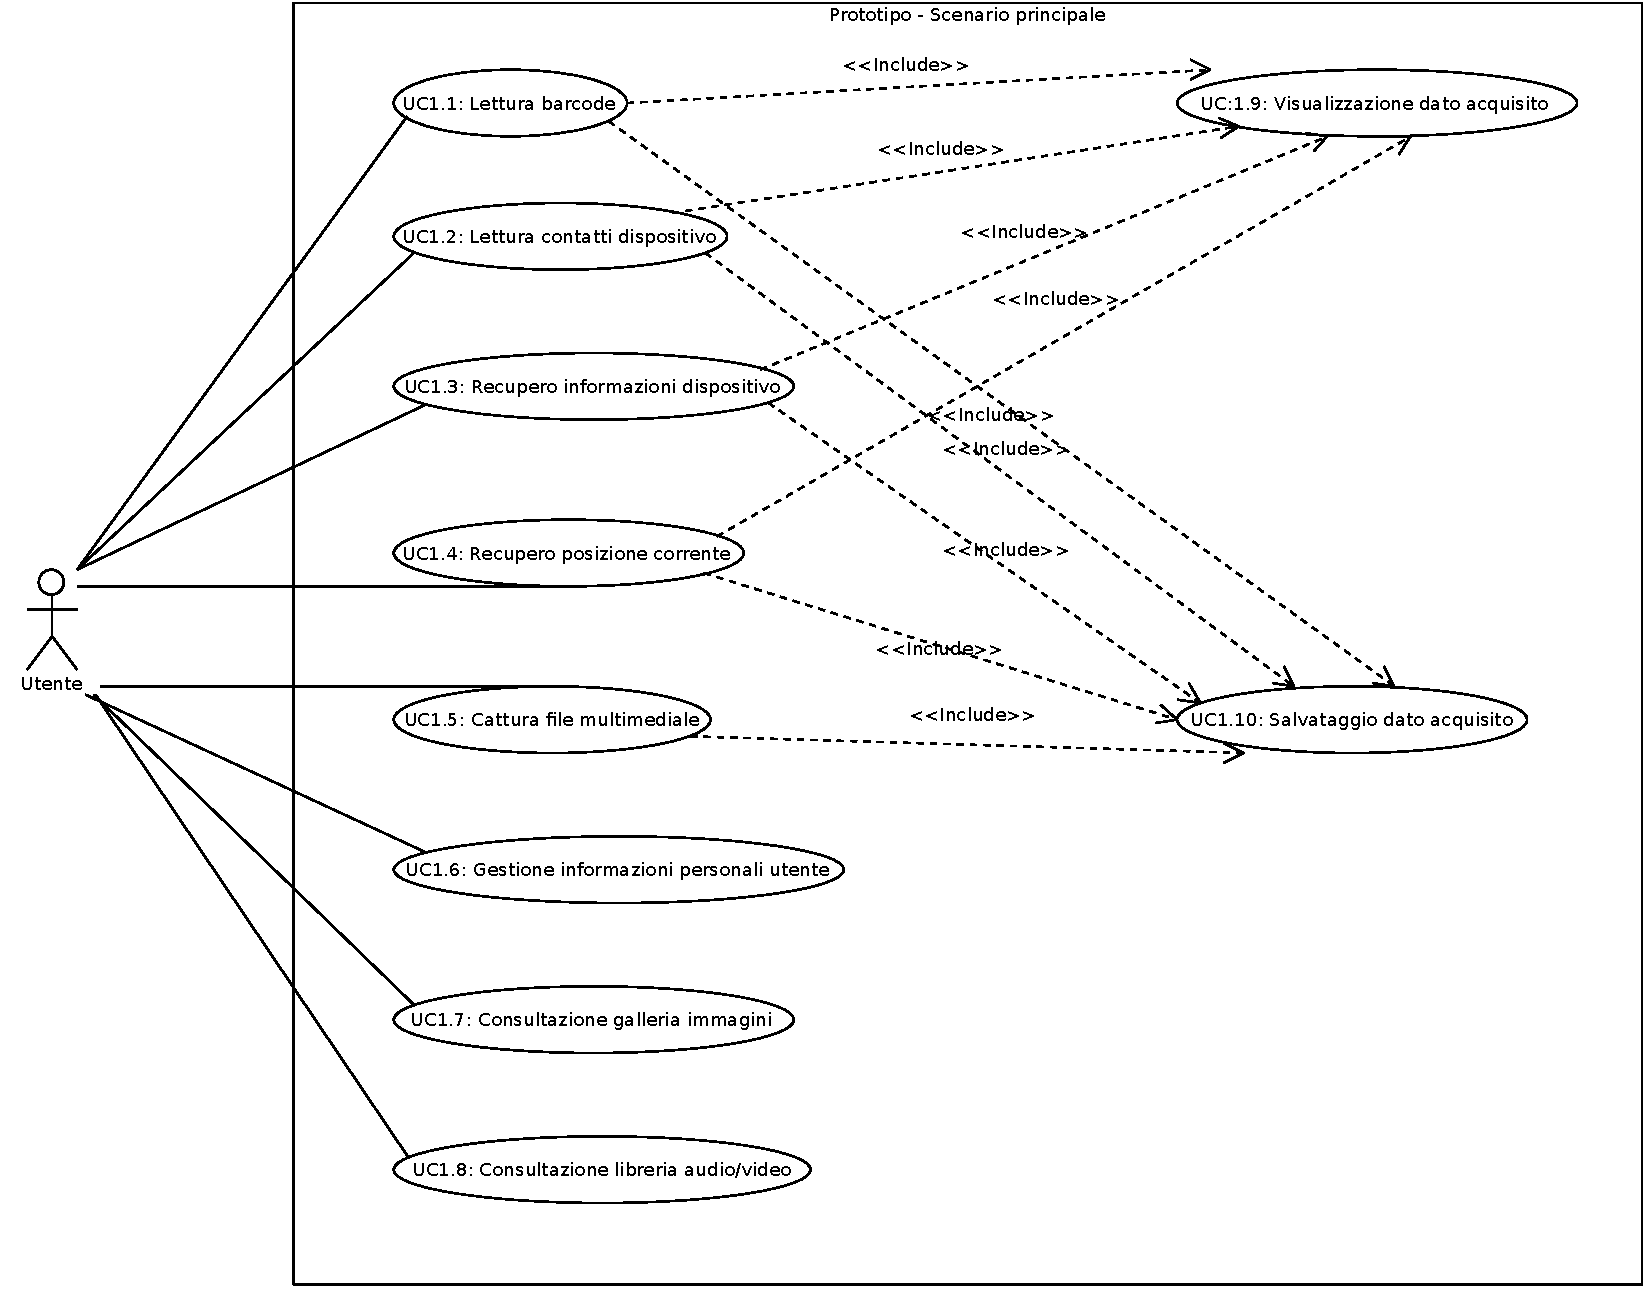
\includegraphics[scale=0.45]{gfx/useCase/UC1_Scenario_principale.pdf}
\caption{Caso d'uso UC1: Scenario principale}
\label{fig:UC1}
\end{figure}

\begin{description}
\item[attori:] Utente;
\item[scopo e descrizione:] L'utente ha avviato correttamente l'applicazione e questa è pronta all'uso. Egli può effettuare varie operazioni: leggere codici a barre, recuperare i contatti del dispositivo, recuperare le informazioni del dispositivo, catturare file multimediali, recuperare la posizione corrente dal \ac{GPS}, gestire le proprie informazioni personali, consultare la galleria immagini e la libreria audio/video, salvare e visualizzare i dati catturati tramite il dispositivo;
\item[precondizione:] L'applicazione è stata avviata ed è pronta all'uso.
\item[flusso principale degli eventi:] \hfill \\
	\begin{enumerate}
	\item L'utente può leggere codici a barre;
	\item L'utente può recuperare i contatti del dispositivo;
	\item L'utente può recuperare le informazioni del dispositivo;
	\item L'utente può catturare file multimediali;
	\item L'utente può recuperare la posizione corrente;
	\item L'utente può gestire le proprie informazioni personali;
	\item L'utente può consultare la galleria;
	\item L'utente può consultare la libreria;
	\end{enumerate}
\item[inclusioni:] \hfill \\
	\begin{enumerate}
	\item Il sistema salva i dati acquisiti;
	\item Il sistema visualizza i dati acquisiti;
	\end{enumerate}
\item[postcondizione:] Il sistema ha ottenuto informazioni sulle operazioni che l'utente vuole eseguire.
\end{description}

\subsection{Caso d'uso UC1.1: Lettura barcode}
\begin{description}
\item[attori:] Utente;
\item[scopo e descrizione:] L'utente ha scelto l'opzione di lettura di un codice a barre;
\item[precondizione:] Il sistema è pronto per la lettura di un nuovo codice;
\item[scenari alternativi:] \hfill \\
	\begin{enumerate}
	\item L'utente decide di annullare l'operazione di lettura; il sistema torna allo stato precedente la scelta dell'utente;
	\end{enumerate}
\item[postcondizione:] Il sistema ha letto il codice e procede con il salvataggio e la visualizzazione dei dati.
\end{description}

\subsection{Caso d'uso UC1.2: Cattura file multimediale}
\begin{figure}[htb]
\centering
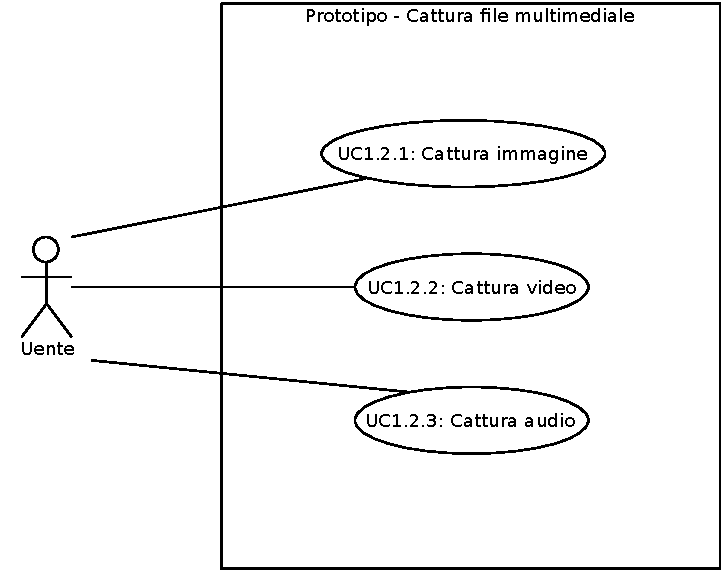
\includegraphics[scale=0.6]{gfx/useCase/UC1-2_Cattura_file_multimediale.pdf}
\caption{Caso d'uso UC1.2: Cattura file multimediale}
\label{fig:UC1.2}
\end{figure}

\begin{description}
\item[attori:] Utente;
\item[scopo e descrizione:] L'utente ha scelto l'opzione di cattura di un file multimediale e può decidere quale tipo di file catturare: immagine, audio o video;
\item[precondizione:] Il sistema mostra le possibili scelte all'utente;
\item[flusso principale degli eventi:] \hfill \\
	\begin{enumerate}
	\item L'utente può catturare un'immagine;
	\item L'utente può catturare un video;
	\item L'utente può catturare un file audio;
	\end{enumerate}
\item[postcondizione:] Il sistema è pronto per la cattura del file multimediale prescelto.
\end{description}

\subsection{Caso d'uso UC1.2.1: Cattura immagine}
\begin{figure}[htb]
\centering
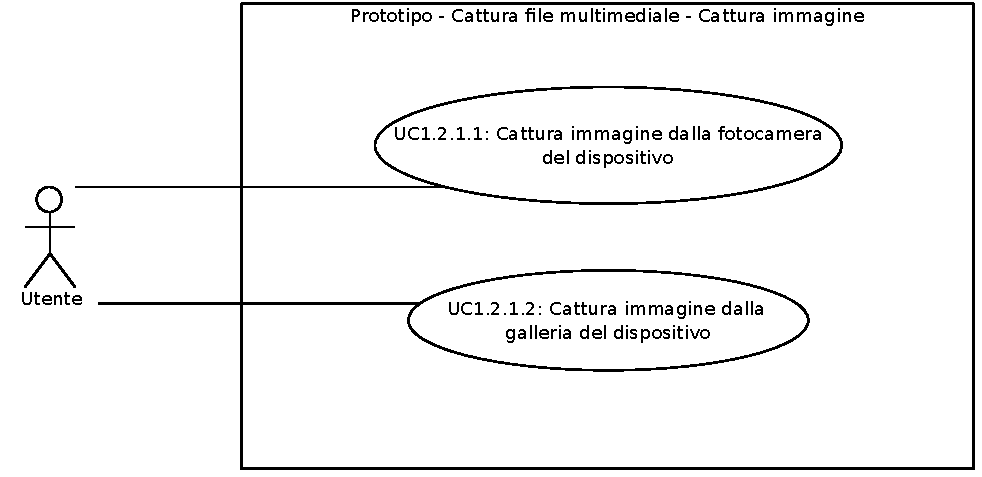
\includegraphics[scale=0.6]{gfx/useCase/UC1-2-1_Cattura_immagine.pdf}
\caption{Caso d'uso UC1.2.1: Cattura immagine}
\label{fig:UC1.2}
\end{figure}

\begin{description}
\item[attori:] Utente;
\item[scopo e descrizione:] L'utente ha scelto l'opzione di cattura di un'immagine e può scegliere se utilizzare la fotocamera del dispositivo oppure la galleria dello stesso;
\item[precondizione:] Il sistema mostra le possibili scelte all'utente;
\item[flusso principale degli eventi:] \hfill \\
	\begin{enumerate}
	\item L'utente può catturare un'immagine dalla fotocamera del dispositivo;
	\item L'utente può catturare un'immagine dalla galleria del dispositivo;
	\end{enumerate}
\item[postcondizione:] Il sistema è pronto per la cattura dell'immagine dalla fonte prescelta.
\end{description}

\subsection{Caso d'uso UC1.2.2: Cattura immagine dalla fotocamera del dispositivo}
\begin{description}
\item[attori:] Utente;
\item[scopo e descrizione:] L'utente ha scelto la cattura di un'immagine dalla fotocamera del dispositivo;
\item[precondizione:] Il sistema è pronto per la cattura di una nuova immagine dalla fotocamera;
\item[scenari alternativi:] \hfill \\
	\begin{enumerate}
	\item L'utente decide di annullare l'operazione di cattura; il sistema torna allo stato precedente la scelta dell'utente;
	\end{enumerate}
\item[postcondizione:] Il sistema ha catturato una nuova immagine e procede con il salvataggio.
\end{description}

\subsection{Caso d'uso UC1.2.2: Cattura immagine dalla galleria del dispositivo}
\begin{description}
\item[attori:] Utente;
\item[scopo e descrizione:] L'utente ha scelto la cattura di un'immagine dalla galleria del dispositivo;
\item[precondizione:] Il sistema è pronto per la cattura di una nuova immagine dalla galleria;
\item[scenari alternativi:] \hfill \\
	\begin{enumerate}
	\item L'utente decide di annullare l'operazione di cattura; il sistema torna allo stato precedente la scelta dell'utente;
	\end{enumerate}
\item[postcondizione:] Il sistema ha catturato una nuova immagine e procede con il salvataggio.
\end{description}

\subsection{Caso d'uso UC1.2.2: Cattura video}
\begin{description}
\item[attori:] Utente;
\item[scopo e descrizione:] L'utente ha scelto la cattura di un video;
\item[precondizione:] Il sistema è pronto per la cattura di un nuovo video;
\item[scenari alternativi:] \hfill \\
	\begin{enumerate}
	\item L'utente decide di annullare l'operazione di cattura; il sistema torna allo stato precedente la scelta dell'utente;
	\end{enumerate}
\item[postcondizione:] Il sistema ha catturato una nuovo video e procede con il salvataggio.
\end{description}

\subsection{Caso d'uso UC1.2.3: Cattura audio}
\begin{description}
\item[attori:] Utente;
\item[scopo e descrizione:] L'utente ha scelto la cattura di un file audio;
\item[precondizione:] Il sistema è pronto per la cattura di una nuovo file audio;
\item[scenari alternativi:] \hfill \\
	\begin{enumerate}
	\item L'utente decide di annullare l'operazione di cattura; il sistema torna allo stato precedente la scelta dell'utente;
	\end{enumerate}
\item[postcondizione:] Il sistema ha catturato una nuovo file audio e procede con il salvataggio.
\end{description}

\subsection{Caso d'uso UC1.3: Recupero informazioni dispositivo}
\begin{description}
\item[attori:] Utente;
\item[scopo e descrizione:] L'utente ha scelto il recupero delle informazione del dispositivo;
\item[precondizione:] Il sistema è pronto per il recupero delle informazioni;
\item[postcondizione:] Il sistema ha recuperato le informazioni e procede con il salvataggio e la visualizzazione.
\end{description}

\subsection{Caso d'uso UC1.4: Recupero posizione corrente}
\begin{description}
\item[attori:] Utente,
\item[scopo e descrizione:] L'utente ha scelto il recupero della posizione corrente tramite il \ac{GPS} del dispositivo;
\item[precondizione:] Il sistema è pronto per il recupero della posizione;
\item[postcondizione:] Il sistema ha recuperato la posizione del dispositivo e procede con il salvataggio e la visualizzazione.
\end{description}

\subsection{Caso d'uso UC1.5: Lettura contatti dispositivo}
\begin{description}
\item[attori:] Utente;
\item[scopo e descrizione:] L'utente ha scelto la lettura dei contatti dal dispositivo;
\item[precondizione:] Il sistema è pronto per la lettura dei contatti presenti nel dispositivo;
\item[postcondizione:] Il sistema ha recuperato i contatti del dispositivo e procede con il salvataggio e la visualizzazione.
\end{description}

\subsection{Caso d'uso UC1.6: Gestione informazioni personali utente}
\begin{figure}[htb]
\centering
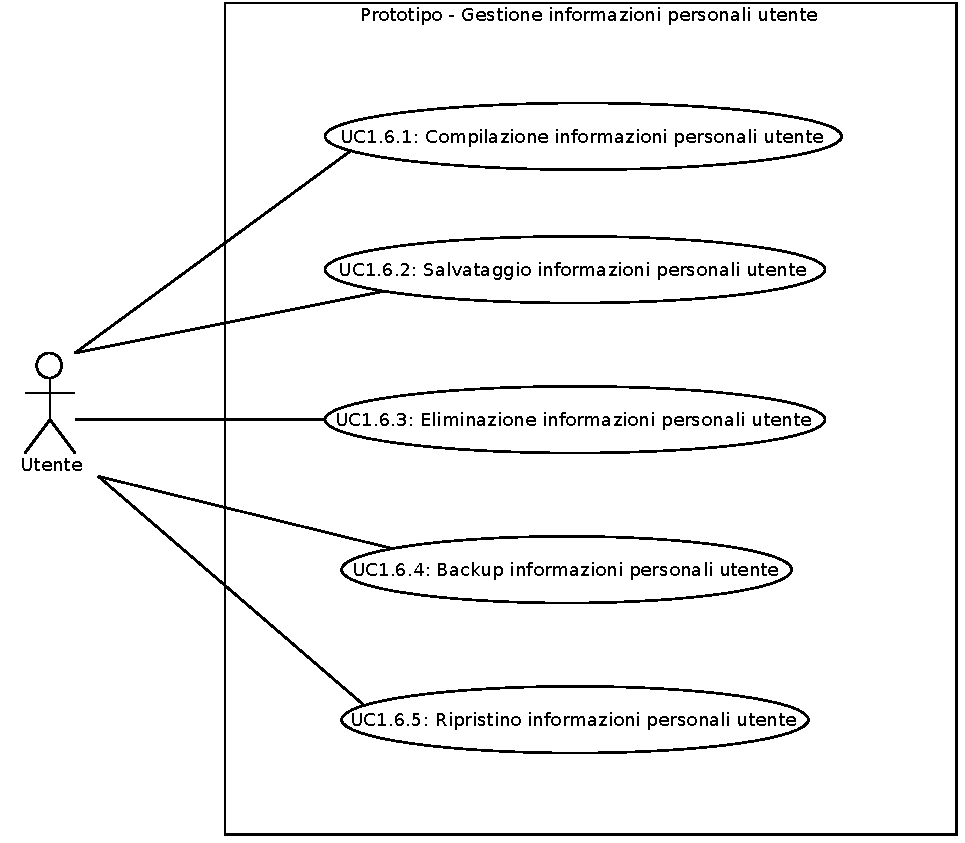
\includegraphics[scale=0.6]{gfx/useCase/UC1-6_Gestione_informazioni_personali_utente.pdf}
\caption{Caso d'uso UC1.6: Gestione informazioni personali utente}
\label{fig:UC1.6}
\end{figure}

\begin{description}
\item[attori:] Utente;
\item[scopo e descrizione:] L'utente ha scelto la gestione delle informazioni personali e può procedere con la compilazione di tali informazioni oppure salvare, eliminare, effettuare un backup o un ripristino di tali dati;
\item[precondizione:] Il sistema è pronto per gestire le informazioni personali dell'utente;
\item[flusso principale degli eventi:] \hfill \\
	\begin{enumerate}
	\item L'utente può compilare le informazioni personali;
	\item L'utente può salvare le informazioni personali;
	\item L'utente può eliminare le informazioni personali;
	\item L'utente può effettuare un backup delle informazioni personali;
	\item L'utente può effettuare un ripristino delle informazioni personali;
	\end{enumerate}
\item[postcondizione:] Il sistema è pronto ad eseguire l'opzione scelta dell'utente;
\end{description}

\subsection{Caso d'uso UC1.6.1: Compilazione informazioni personali utente}
\begin{description}
\item[attori:] Utente;
\item[scopo e descrizione:] L'utente ha scelto di compilare le informazioni personali;
\item[precondizione:] Il sistema è pronto per accettare l'immissione delle informazioni dell'utente;
\item[postcondizione:] Il sistema ha scritto le informazioni immesse dall'utente.
\end{description}

\subsection{Caso d'uso UC1.6.2: Salvataggio informazioni personali utente}
\begin{description}
\item[attori:] Utente;
\item[scopo e descrizione:] L'utente ha scelto di salvare le informazioni personali immesse;
\item[precondizione:] Il sistema è in possesso delle informazioni immesse dall'utente;
\item[postcondizione:] Il sistema ha salvato le informazioni immesse dall'utente.
\end{description}

\subsection{Caso d'uso UC1.6.3: Eliminazione informazioni personali utente}
\begin{description}
\item[attori:] Utente;
\item[scopo e descrizione:] L'utente ha scelto di eliminare le informazioni salvate;
\item[precondizione:] Il sistema possiede le informazioni dell'utente ed è pronto ad eliminarle;
\item[postcondizione:] Il sistema ha eliminato le informazioni dell'utente.
\end{description}

\subsection{Caso d'uso UC1.6.4: Backup informazioni personali utente}
\begin{description}
\item[attori:] Utente;
\item[scopo e descrizione:] L'utente ha scelto di effettuare un backup delle informazioni salvate;
\item[precondizione:] Il sistema possiede le informazioni salvate dell'utente ed è pronto al backup;
\item[postcondizione:] Il sistema ha effettuato il backup delle informazioni sulla memoria del dispositivo.
\end{description}

\subsection{Caso d'uso UC1.6.5: Ripristino informazioni personali utente}
\begin{description}
\item[attori:] Utente;
\item[scopo e descrizione:] L'utente ha scelto di ripristinare le informazioni di cui ha effettuato una copia di backup;
\item[precondizione:] Il sistema è pronto a ripristinare le informazioni dell'utente;
\item[postcondizione:] Il sistema a ripristinato le informazioni dell'utente.
\end{description}

\subsection{Caso d'uso UC1.7: Consultazione galleria immagini}
\begin{description}
\item[attori:] Utente;
\item[scopo e descrizione:] L'utente ha scelto di consultare la galleria delle immagini;
\item[precondizione:] Il sistema è pronto a visualizzare la galleria delle immagini;
\item[postcondizione:] Il sistema ha visualizzato la galleria delle immagini.
\end{description}

\subsection{Caso d'uso UC1.8: Consultazione libreria audio/video}
\begin{description}
\item[attori:] Utente;
\item[scopo e descrizione:] L'utente ha scelto di consultare la libreria audio/video;
\item[precondizione:] Il sistema è pronto a visualizzare la libreria audio/video;
\item[postcondizione:] Il sistema ha visualizzato la libreria audio/video.
\end{description}

\subsection{Caso d'uso UC1.9: Visualizzazione dato acquisito}
\begin{description}
\item[attori:] Sistema;
\item[scopo e descrizione:] Il sistema visualizza il dato acquisito;
\item[precondizione:] Il sistema è pronto a visualizzare il dato acquisito;
\item[postcondizione:] Il sistema ha visualizzato il dato acquisito.
\end{description}

\subsection{Caso d'uso UC1.10: Salvataggio dato acquisito}
\begin{description}
\item[attori:] Sistema;
\item[scopo e descrizione:] Il sistema salva il dato acquisito;
\item[precondizione:] Il sistema è pronto a visualizzare il dato acquisito;
\item[postcondizione:] Il sistema ha salvato il dato acquisito.
\end{description}

\section{Requisiti}
Di seguito vengono riportati i requisiti individuati dall'analisi effettuata sulle richieste dell'azienda, emersi dai casi d'uso o nati da esigenze interne.

Sono classificati per tipo e importanza secondo la seguente codifica:
\begin{center}
R[importanza][tipo][codice]
\end{center}

\begin{description}
\item[importanza:] \hfill \\
	\setcounter{enumi}{-1}
	\begin{enumerate}
	\item Requisito obbligatorio;
	\item Requisito desiderabile;
	\item Requisito opzionale.
	\end{enumerate}
\item[tipo:] \hfill \\
	\begin{description}
	\item[F:] Funzionale;
	\item[Q:] Di qualità;
	\item[P:] Prestazionale;
	\item[V:] Di vincolo.
	\end{description}
\item[codice:] è il codice univoco di ogni requisito espresso in modo gerarchico.
\end{description}

%************************************************
\chapter{Progettazione}\label{ch:progettazione}
%************************************************
Il seguente capitolo descrive le scelte progettuali che sono state effettuate, ovvero viene presentata l'architettura generale di \emph{Sencha Touch} e dei prototipi \emph{MyNotes} e \emph{SensorDevice} attraverso diagrammi delle classi.

\section{Sencha Touch 2}
JavaScript, il linguaggio con cui è stato scritto il framework \emph{Sencha Touch}, è un linguaggio di scripting prototype-based e multi-paradigma, supporta infatti sia uno stile di programmazione imperativa e object-oriented cheo funzionale.

Tali caratteristiche lo rendono un linguaggio molto flessibile che permette di risolvere lo stesso problema in molti modi e con differenti tecniche; purtroppo la mancanza di struttura nel linguaggio porta il grande svantaggio dell'imprevedibilità.

Inoltre, ogni chiamata a funzione che viene effettuata è asincrona, il che rende ancora meno semplice addomesticare il linguaggio ai propri scopi.

I progettisti di \emph{Sencha Touch} hanno quindi cercato di dare una struttura solida al framework creando una gerarchia di oggetti e modellando attorno ad essi un'architettura \ac{MVC}.

Il risultato ottenuto è che ogni applicazione che si intende sviluppare con tale framework deve seguire correttamente tale pattern per riuscire a sfruttare appieno il sistema di classi messo a punto dai progettisti.

\begin{figure}[htb]
\centering
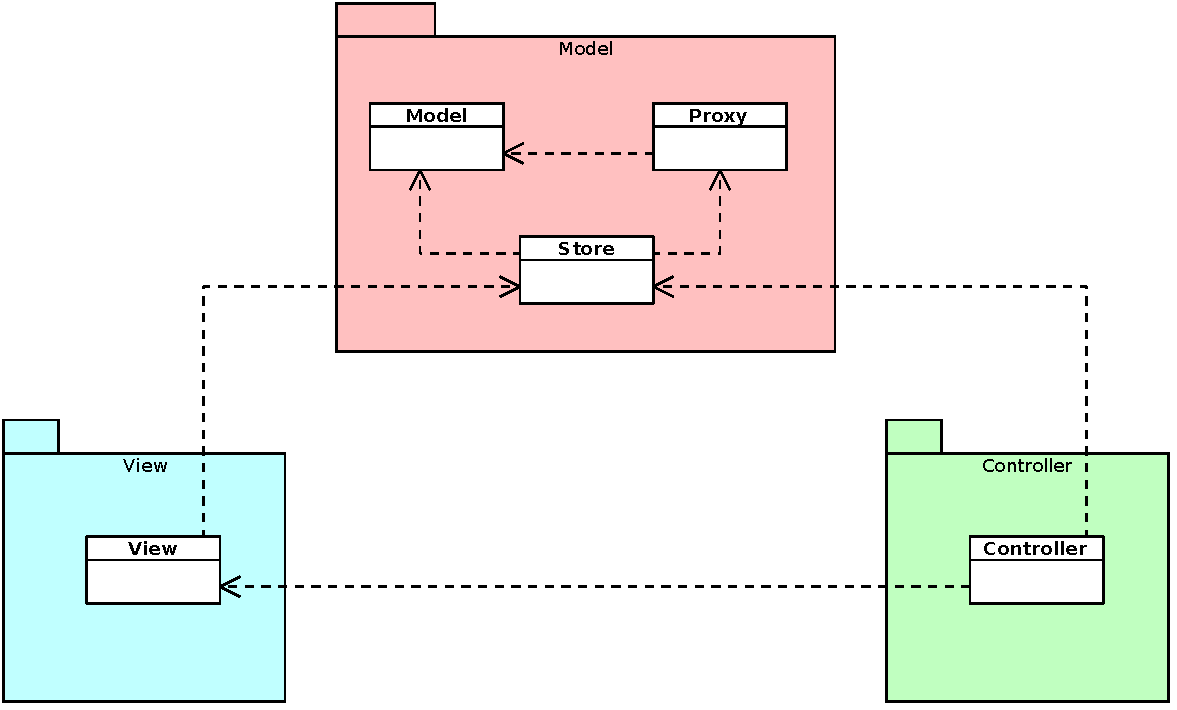
\includegraphics[scale=0.6]{gfx/class/Sencha_Touch_2.pdf}
\caption{Architettura generale Sencha Touch 2}
\label{fig:architettura Sencha}
\end{figure}
Il diagramma in figura \ref{fig:architettura Sencha} rappresenta l'architettura generale che ogni applicazione deve avere, ciò è riflesso anche nella struttura di cartelle e nei nomi dei file; essa si basa sul pattern architetturale \ac{MVC} il quale è composto da 4 package che svolgono funzioni diverse:
\begin{description}
\item[model:] rappresenta il modello dei dati su cui si basa l'applicazione; ogni oggetto \emph{model} viene gestito da uno \emph{store} che si occupa di leggere e scrivere i dati mediante un \emph{proxy};
\item[store:] rappresenta una collezione di istanze di modelli e viene utilizzato per gestire caricamento, modifica e salvataggio dei dati dell'applicazione tramite un \emph{proxy};
\item[view:] rappresenta tutti gli oggetti che servono a visualizzare le informazioni all'utente e si riflette dunque sull'interfaccia grafica;
\item[controller:] rappresenta il gestore della logica dell'applicazione; esegue il collegamento tra l'azione che l'utente desidera svolgere e i dati effettivi sul quale l'azione deve essere eseguita.
\end{description}

\section{MyNotes}
\begin{figure}[htbp]
\centering
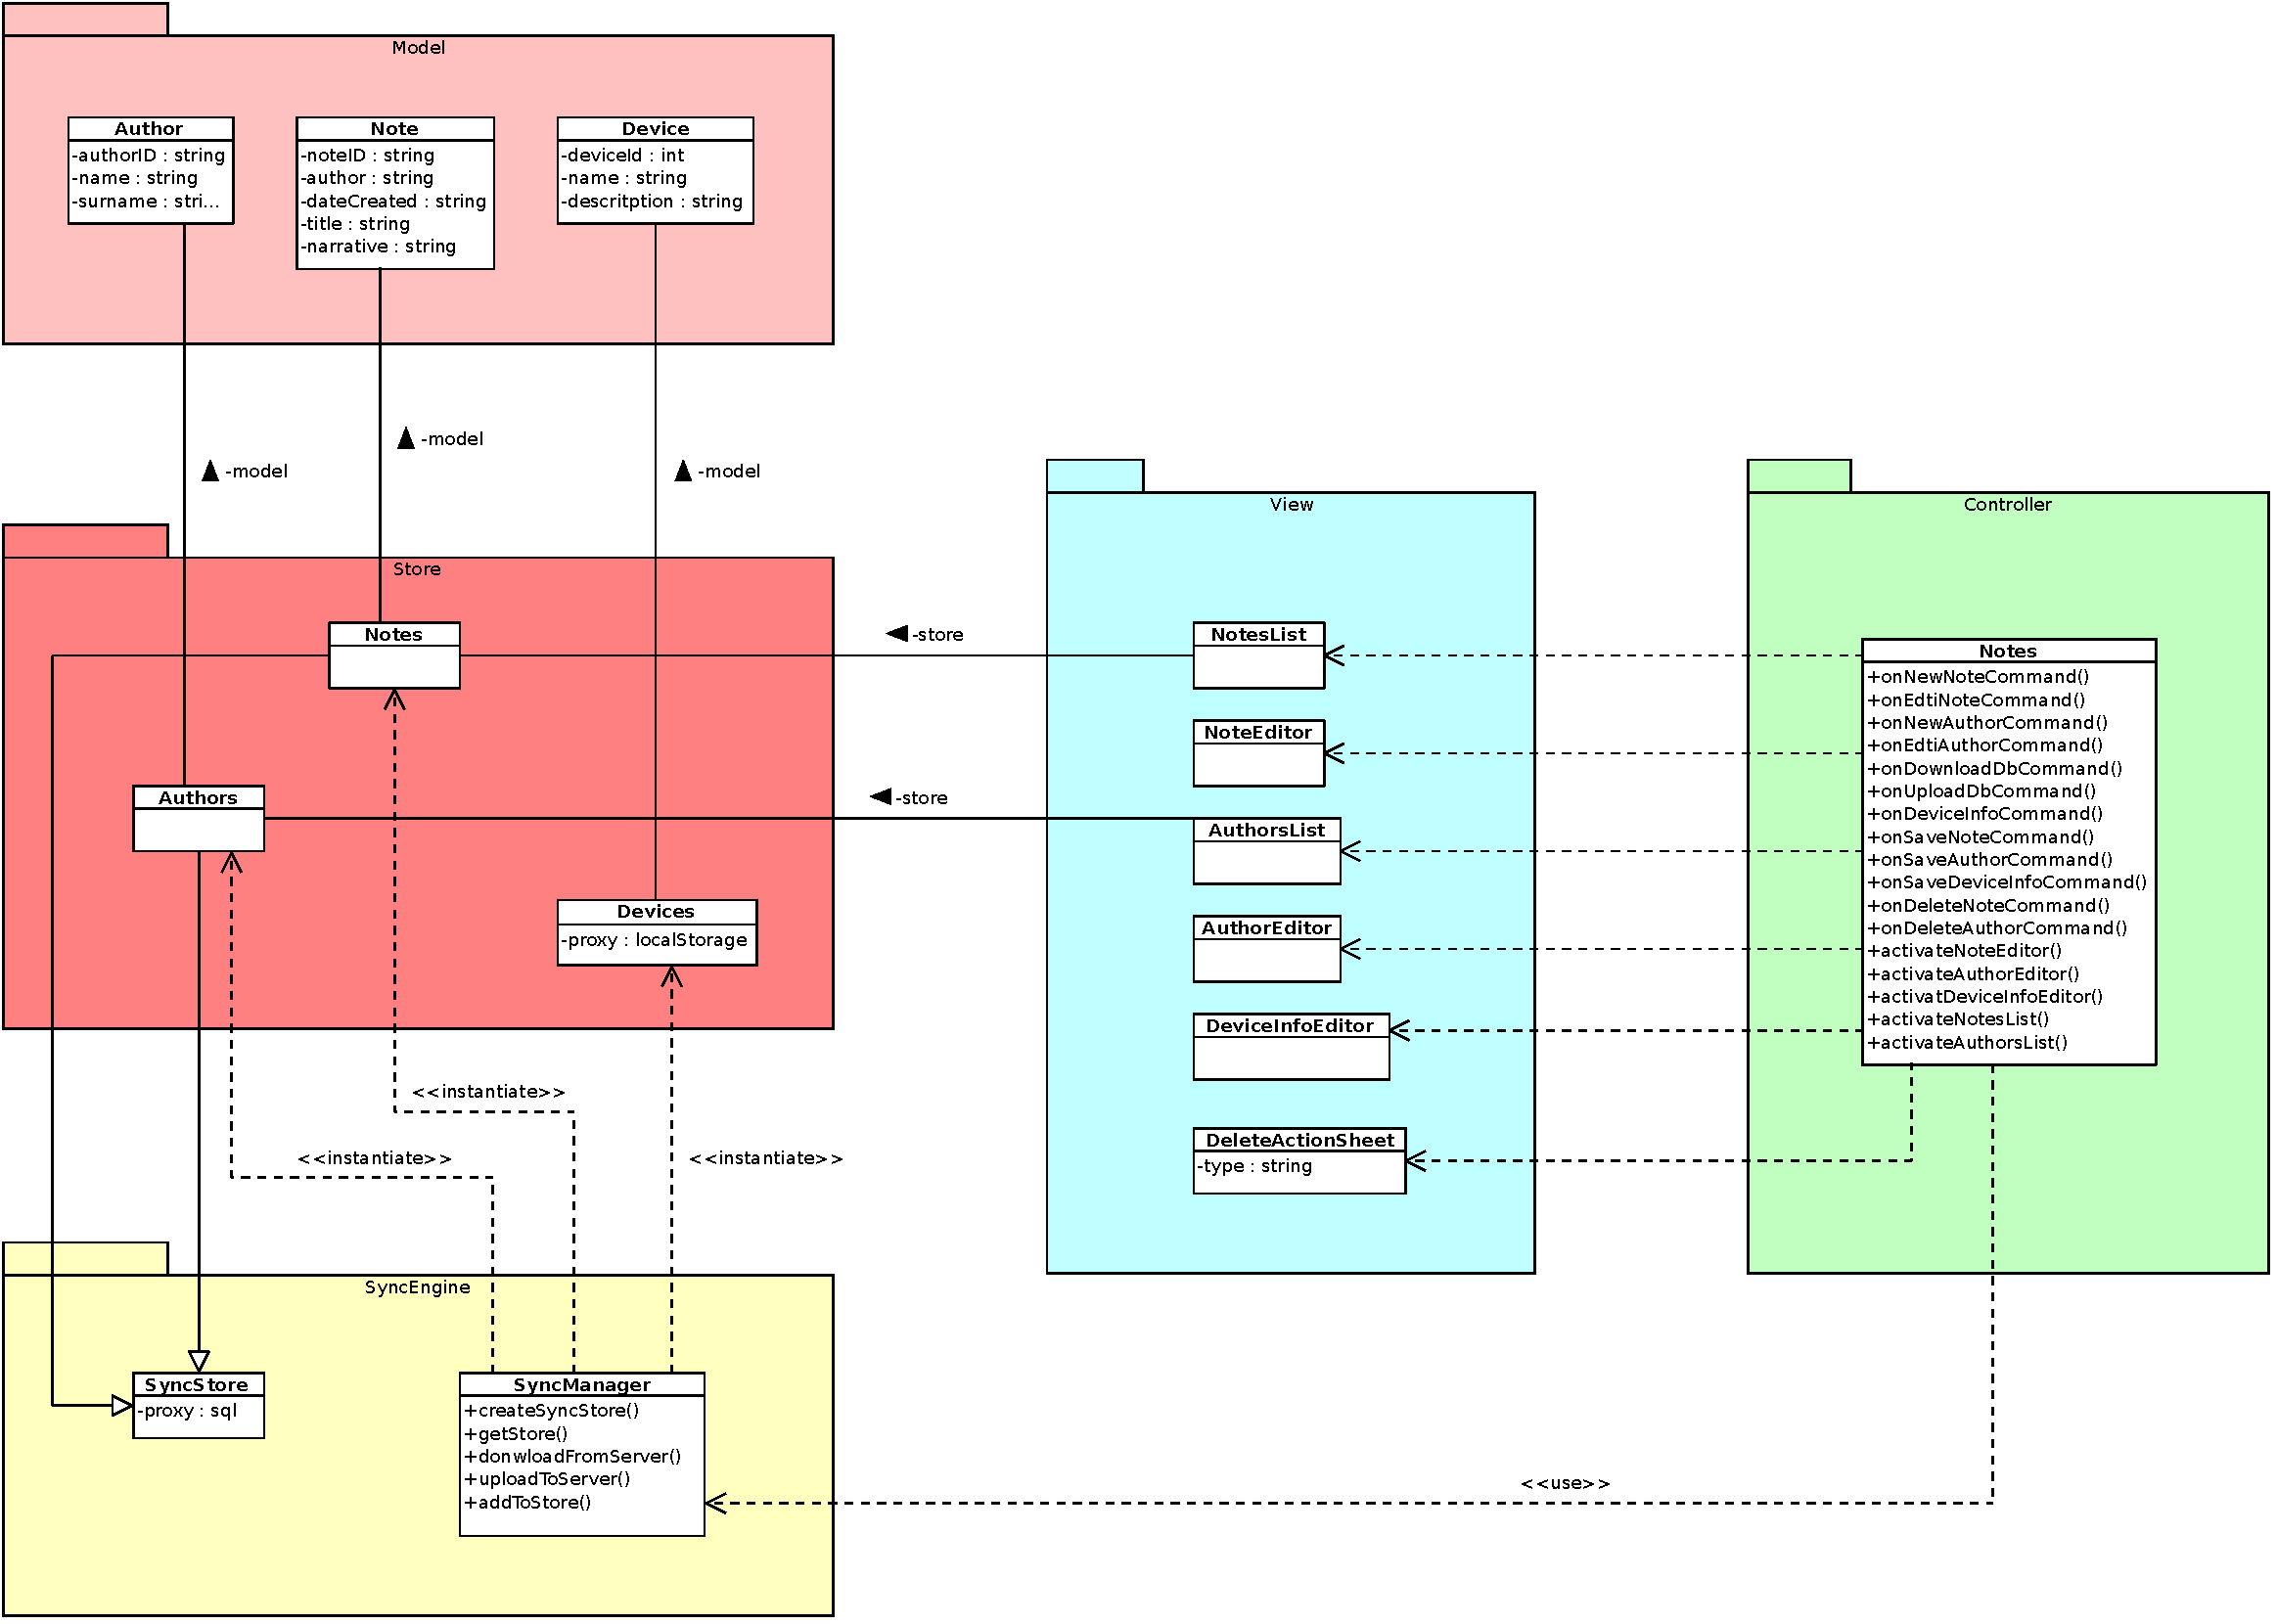
\includegraphics[scale=0.5,angle=90]{gfx/class/MyNotes.pdf}
\caption{Architettura generale -- MyNotes}
\label{fig:architettura MyNotes}
\end{figure}
L'architettura generale dell'applicazione \emph{MyNotes} è rappresentata in figura \ref{fig:architettura MyNotes} ed evidenzia le dipendenze esistenti tra i package individuati.

Dal diagramma si evince come non ci siano gerarchie tra i componenti, ma ogni prototipo rappresenta un'entità particolare con compiti specifici che vengono gestiti dal controller; ognuno di questi oggetti, esclusi il controller e il \emph{SyncManager}, interagisce con al più un altro oggetto, il che rende semplice l'organizzazione dei componenti.

\subsection{Model - Store}
\begin{figure}[htb]
\centering
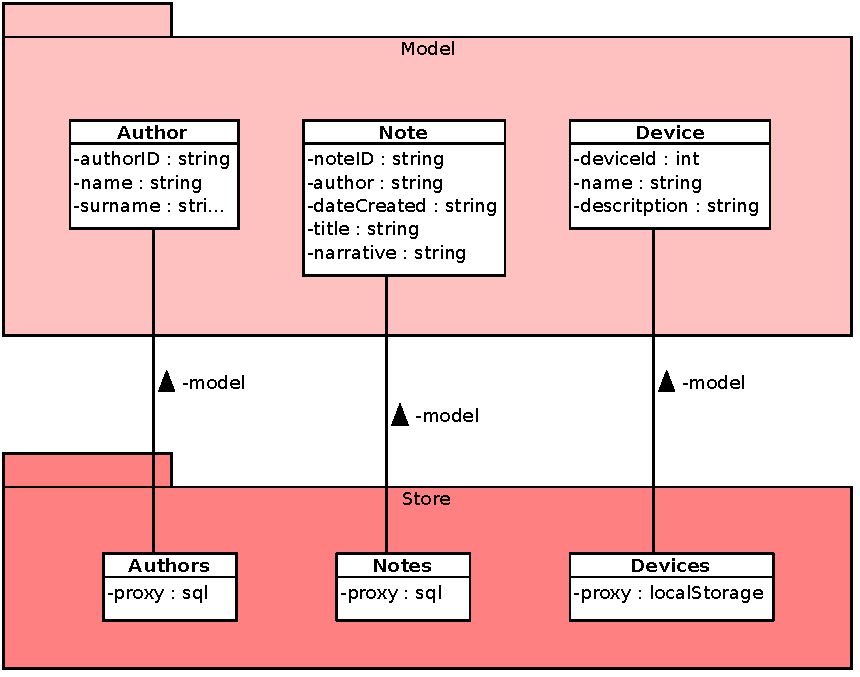
\includegraphics[scale=0.6]{gfx/class/MyNotes_Model_Store.pdf}
\caption{Architettura generale -- MyNotes Model - Store}
\label{fig:architettura MyNotes Model-Store}
\end{figure}
Per soddisfare i requisiti e quindi la necessità di gestire note, autori e device si sono progettati tre modelli omonimi con i relativi store.
I modelli in questione sono molto semplici e contengono pochi campi in quanto non rappresentano un'entità reale ma solo dimostrativo.

Per autori e note si è scelto di utilizzare il proxy di tipo \emph{sql} il quale usa \emph{SQLite} per il salvataggio dei dati; la scelta è stata obbligata in quanto il \emph{SyncManager} utilizza tale tipo di proxy.
Per quanto riguarda le informazioni del dispositivo invece è sufficiente un proxy di tipo \emph{localStorage} in quanto non necessita di essere sincronizzato e può essere gestito localmente.

\subsection{View}
\begin{figure}[htb]
\centering
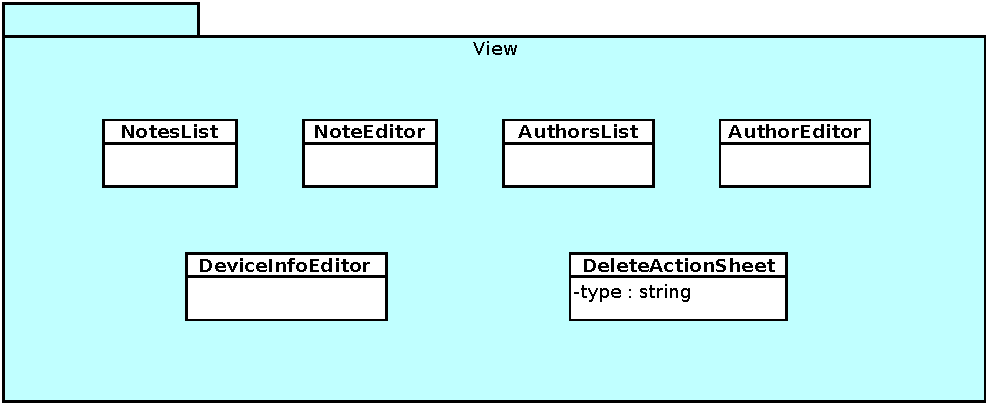
\includegraphics[scale=0.6]{gfx/class/MyNotes_View.pdf}
\caption{Architettura generale -- MyNotes View}
\label{fig:architettura MyNotes View}
\end{figure}
Le viste progettate sono dei componenti che vengono utilizzati per visualizzare la lista delle note, \emph{NotesList}, e degli autori, \emph{AuthorsList} e per gestire creazione e modifica di note, \emph{NoteEditor}, autori, \emph{AuthorEditor}, e delle informazioni del dispositivo, \emph{DeviceInfoEditor}.

È presente un ulteriore vista, \emph{DeleteActionSheet}, che ha il compito di richiedere la conferma dell'eliminazione di una nota o di un autore all'utente; tale componente è in grado di distinguere il tipo del dato che l'utente desidera eliminare tramite il parametro \emph{type}.

\subsection{Controller}
\begin{figure}[htb]
\centering
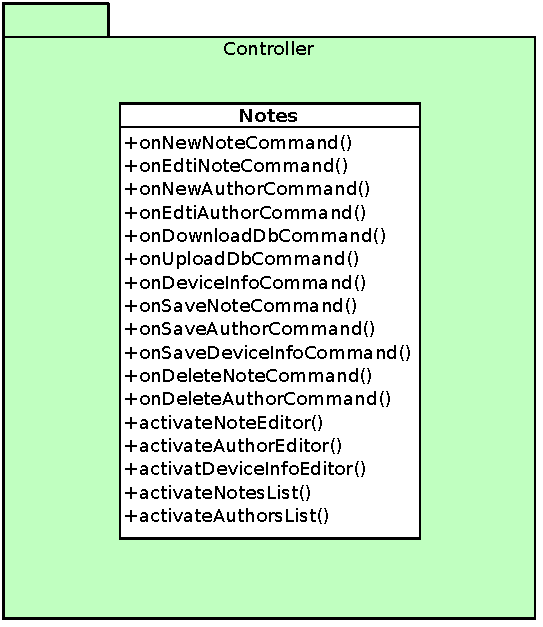
\includegraphics[scale=0.6]{gfx/class/MyNotes_Controller.pdf}
\caption{Architettura generale -- MyNotes Controller}
\label{fig:architettura MyNotes Controller}
\end{figure}
Il \emph{Controller} è il componente più significativo dell'applicazione e viene utilizzato per catturare tutti gli eventi generati dalle viste all'interazione dell'utente con un componente grafico.

Esso infatti dispone dei riferimenti a tutte le viste esistenti ed utilizza dei metodi di controllo per svolgere le diverse operazioni di caricamento, elaborazione e salvataggio dei dati.

Inoltre svolge il suo compito in stretta relazione con il \emph{SyncManager} per quanto riguarda la gestione degli store, infatti, ogni operazione su di essi è mediata da questo componente che svolge la funzione di intermediario con il \emph{SyncEngine} rendendo trasparente allo sviluppatore la gestione dei dati.

\subsection{SyncEngine}
\begin{figure}[htb]
\centering
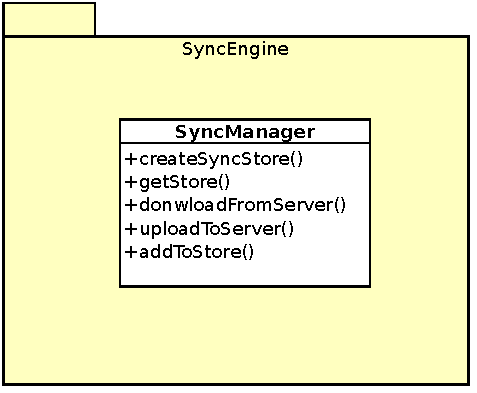
\includegraphics[scale=0.6]{gfx/class/SyncEngine.pdf}
\caption{Architettura generale -- MyNotes SyncEngine}
\label{fig:architettura MyNotes SyncEngine}
\end{figure}
Il \emph{SyncEngine} è un componente che permette di creare dinamicamente degli store legati a modelli statici presenti nell'applicazione, con lo scopo di sincronizzarli con un server remoto adeguatamente predisposto.

Per gestire ed utilizzare correttamente questo componente è stata predisposta un'interfaccia denominata \emph{SyncManager} dalla quale è possibile creare gli store necessari e utilizzarli in modo ottimale all'interno dell'applicazione: sarà quindi possibile utilizzarli per leggere e salvare i dati e per effettuare la sincronizzazione con quelli presenti nel server.

\section{SensorDevice}
\begin{figure}[htb]
\centering
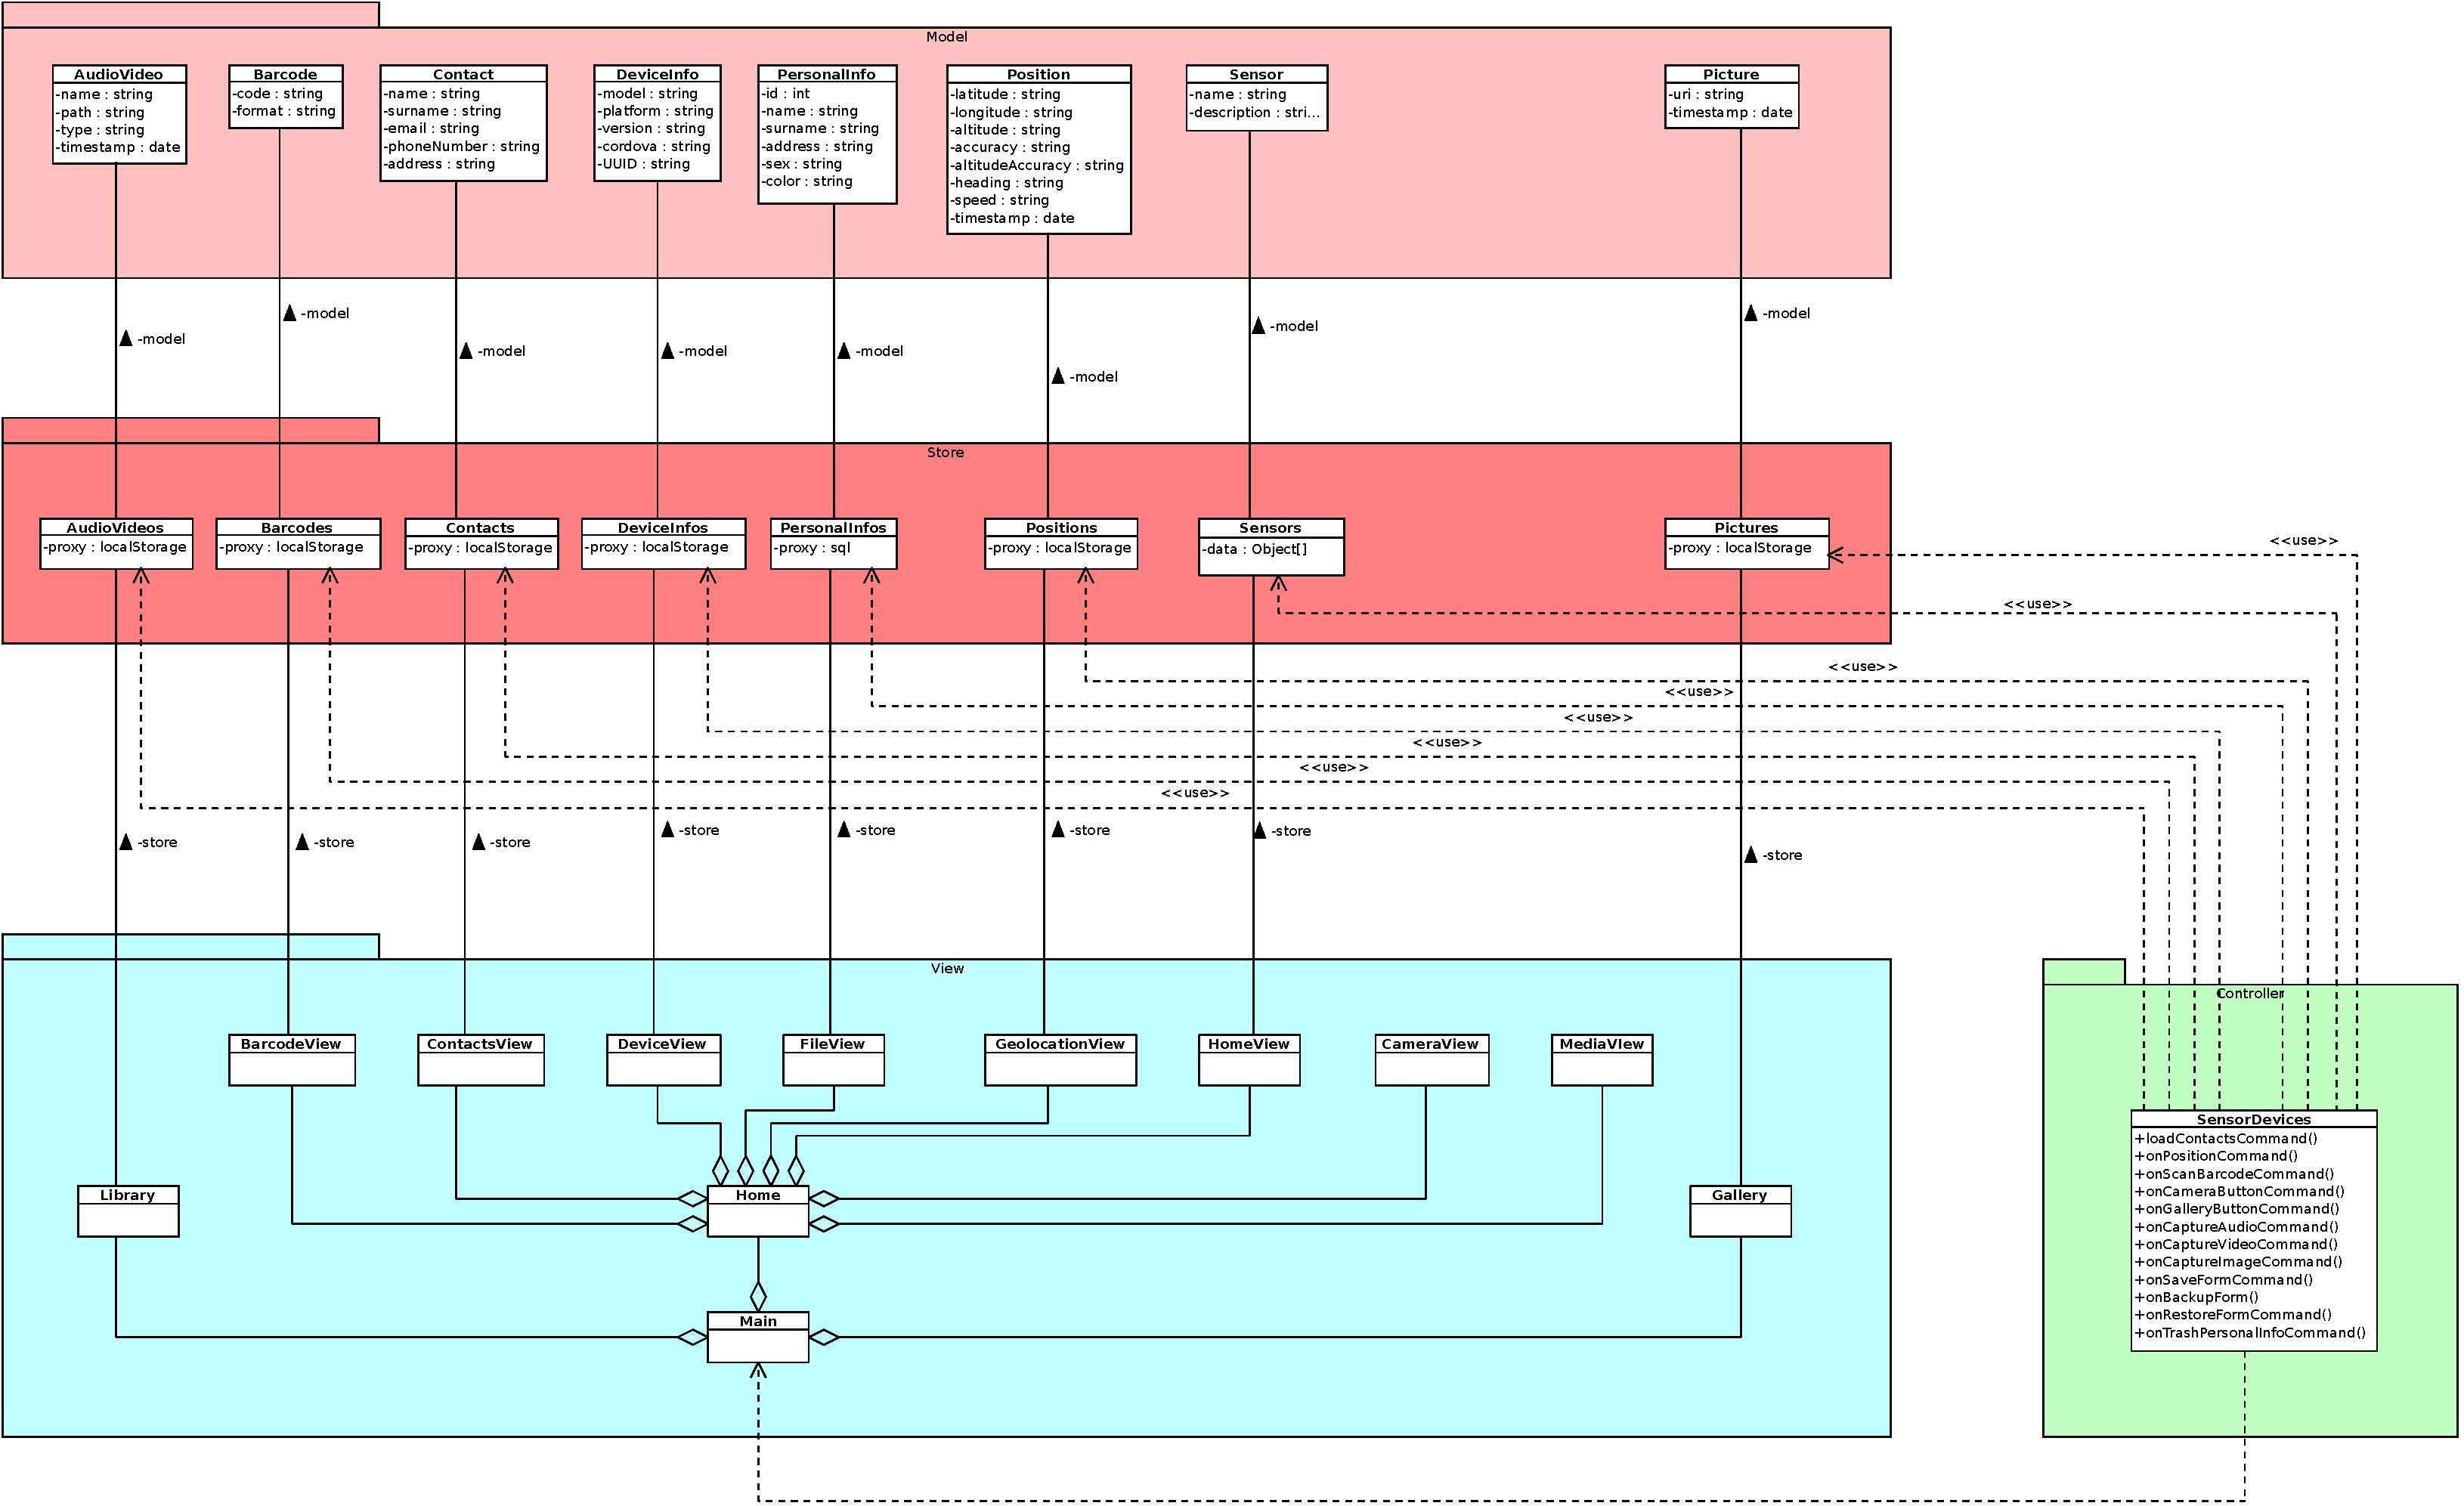
\includegraphics[scale=0.4,angle=90]{gfx/class/SensorDevice.pdf}
\caption{Architettura generale -- SensorDevice}
\label{fig:architettura SensorDevice}
\end{figure}
In figura \ref{fig:architettura SensorDevice} è rappresentata l'architettura ad alto livello dell'applicazione \emph{SensorDevice}: utilizza il pattern architetturale \ac{MVC} che contraddistingue tutte le applicazioni sviluppate con \emph{Sencha Touch}.

Come per \emph{MyNotes} non esistono gerarchie di tipi e il rapporto tra modelli e store è sempre di 1 a 1; si può notare, inoltre, come le viste siano particolarmente articolate a causa della necessità di visualizzare una notevole quantità di dati che vengono raccolti dal sistema.

\subsection{Model - Store}
\begin{figure}[htb]
\centering
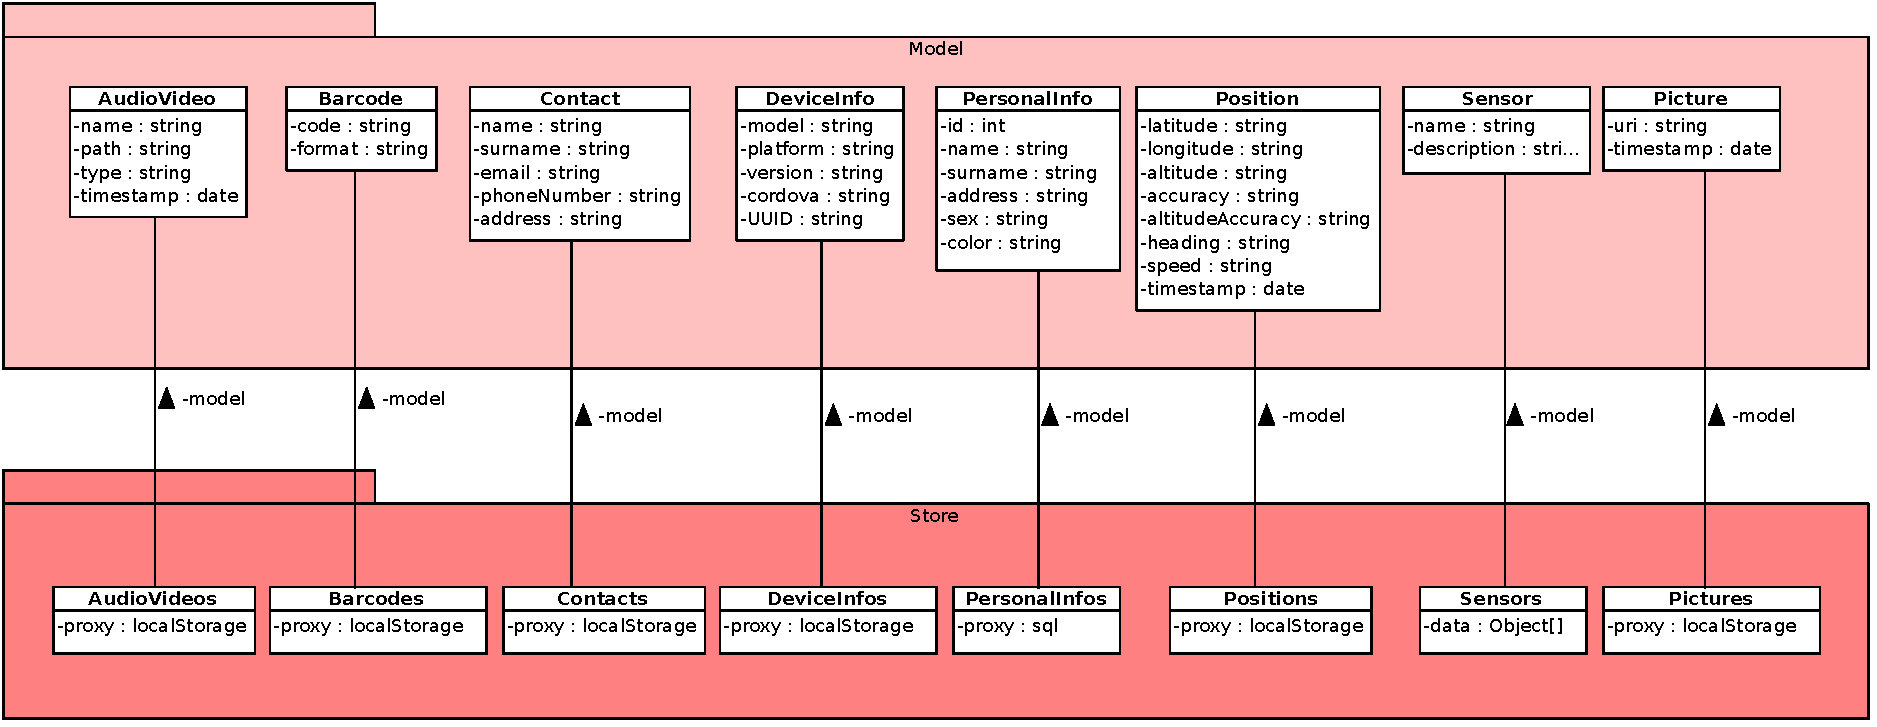
\includegraphics[scale=0.4]{gfx/class/SensorDevice_Model_Store.pdf}
\caption{Architettura generale -- SensorDevice Model - Store}
\label{fig:architettura SensorDevice Model-Store}
\end{figure}
Per soddisfare le richieste dell'azienda sono stati progettati sette modelli diversi, ognuno rappresentante della funzionalità da sviluppare, più il modello \emph{Sensor} che viene utilizzato solamente per creare una lista delle funzionalità che l'utente può decidere di utilizzare nella pagina principale dell'applicazione.

Ogni modello ha associato uno store con proxy di tipo \emph{localStorage}, tranne \emph{PersonalInfos} che ne possiede uno di tipo \emph{sql}, in quanto, tramite il relativo modello, si intende testare il backup e il ripristino dei dati sulla memoria di massa del dispositivo che verrà effettuato tramite un file di testo.

\subsection{View}
\begin{figure}[htb]
\centering
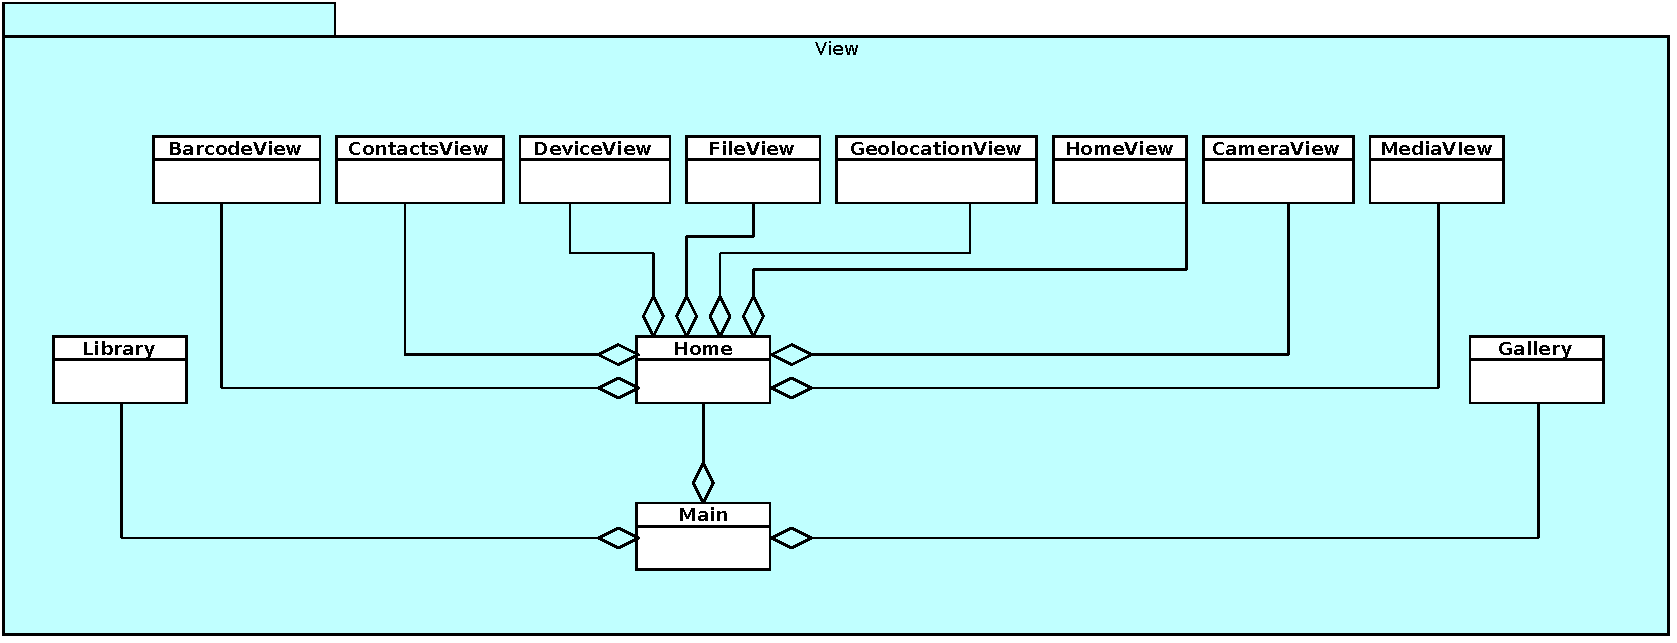
\includegraphics[scale=0.45]{gfx/class/SensorDevice_View.pdf}
\caption{Architettura generale -- SensorDevice View}
\label{fig:architettura SensorDevice View}
\end{figure}
Come si evince dalla figura \ref{fig:architettura SensorDevice View} si è scelto di creare una vista per ogni funzionalità da sviluppare, in modo da rendere più agevole all'utente la consultazione dei dati catturati, e di raggruppare queste in una pagina principale, chiamata \emph{Home}, dalla quale è possibile navigare tutte le viste.

Inoltre sono state progettate due pagine dedicate alla visualizzazione di immagini, \emph{Gallery}, e di video e audio, \emph{Library}.
Si è deciso di dividere le due categorie di \emph{media} in quanto necessitano di una diversa gestione per essere visualizzati o riprodotti.

\subsection{Controller}
\begin{figure}[htb]
\centering
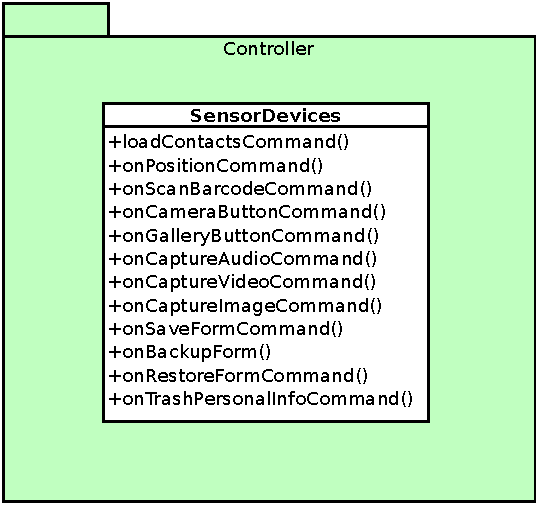
\includegraphics[scale=0.6]{gfx/class/SensorDevice_Controller.pdf}
\caption{Architettura generale -- SensorDevice Controller}
\label{fig:architettura SensorDevice Controller}
\end{figure}
Come per \emph{MyNotes}, il controller possiede riferimenti alle viste dell'applicazione e cattura gli eventi da loro generati, i quali vengono gestiti mediante i metodi predisposti.

In questa applicazione il controller gestisce direttamente creazione e modifica degli store in quanto non è presente nessun componente intermedio come accade per \emph{MyNotes}.
%************************************************
\chapter{Sviluppo}\label{ch:sviluppo}
%************************************************
Il presente capitolo illustra come si è svolto il processo di sviluppo dei prototipi progettati, le problematiche riscontrate e le soluzioni che sono state applicate per risolverle.

La formazione iniziale sui framework da utilizzare è stata svolta su numerose e variegate fonti e con l'ausilio del tutor aziendale e di forum di supporto che hanno semplificato tale apprendimento e hanno contribuito a risolvere dubbi e difficoltà di vario genere.

Una lista esaustiva di tali fonti è da ricercarsi nella \hyperref[app:bibliography]{bibliografia}.

\section{MyNotes}
Lo sviluppo dell'applicazione \emph{MyNotes} ha richiesto uno studio approfondito del modulo \emph{SyncEngine}, tanto per comprenderne il funzionamento quanto per poterne implementarne le funzionalità all'interno dell'applicazione sviluppata.

\subsection{Studio SyncEngine}
Tale componente ha il compito di creare dinamicamente degli store da utilizzare per la gestione dei rispettivi modelli e di sincronizzare i dati inseriti dall'utente con un server predisposto.
Un punto critico di tale sistema è la potenziale distribuzione delle informazioni su più dispositivi; questo comporta l'unione dei dati in possesso di diversi utenti su di un unico database centralizzato in fase di upload e i possibili conflitti sui dati in fase di download a causa della presenza su di un device di dati locali non sincronizzati.

Il problema principale è stata la gestione degli ID dei record e le modifiche ai dati effettuabili da diversi utenti.
Il primo problema è stato parzialmente risolto con l'assegnamento di un codice identificativo ad ogni device, in modo da rendere unici i dati creati da ogni utente.
Il secondo ha richiesto la progettazione di un sistema ad hoc che utilizza store multipli per gestire l'unione dei record presenti nel database remoto con quelli locali in modo di garantire la consistenza globale dei dati.

Lo studio del \emph{SyncEngine} ha portato alla luce alcuni bug presenti in questo componente che non erano stati risolti dallo sviluppatore che ne ha curato la realizzazione:
\begin{itemize}
\item Il codice identificativo del device era cablato nel codice e, quindi, unico per tutte le installazioni dell'applicazione; si sono proposte due alternative:
	\begin{itemize}
	\item La creazione di una pagina dedicata alle informazioni del device in uso da compilare al primo avvio e dalla quale creare un ID univoco;
	\item L'utilizzo di un plugin di Apache Cordova che recupera l'\ac{UUID} proprio del dispositivo;
	\end{itemize}
\item Gli ID progressivi dei record inseriti vengono aggiunti dal sistema in modo automatico ma, ad ogni nuova installazione partono da $1$; in caso di reinstallazioni del software o di pulizia della cache insorgerebbero problemi di duplicazione di ID. Una soluzione potrebbe essere una richiesta al server per un controllo dell'esistenza dell'ID e l'ultimo codice progressivo utilizzato;
\item Ulteriori variabili cablate che facevano riferimento in modo stretto al prototipo realizzato per testare il componente; sono state modificate e rese parametriche per migliorare il riutilizzo del codice;
\item Nel \emph{SyncManager} erano assenti i metodi per effettuare la sincronizzazione con il server, si è quindi deciso di inserire i 2 metodi senza i quali tale funzionalità era nascosta allo sviluppatore:
	\begin{itemize}
	\item \code{downloadFromServer()};
	\item \code{uploadToServer()};
	\end{itemize}
\end{itemize}

\lstinputlisting[language=Java, caption={Metodi di sincronizzazione inseriti in \emph{SyncManager}}, label={lst:metodi sync manager}]{listings/metodi_sincro.java}

\subsection{Sviluppo interfaccia grafica}
Dopo aver compreso l'utilizzo del \emph{SyncEngine} si è iniziato lo sviluppo dell'applicazione seguendo la progettazione effettuata precedentemente.
Non conoscendo a priori le tecnologie utilizzate si è resa necessaria la consultazione di alcune guide online che trattassero gli argomenti richiesti: \emph{Sencha Touch 2.2.1}~\cite{sencha:touch221} con particolare attenzione al sistema delle classi, alla gestione automatica di getter e setter, al funzionamento generale del framework e all'utilizzo di \emph{Sencha Cmd} per creare lo scheletro dell'applicazione che si può vedere in figura \ref{fig:struttura app sencha touch}.

\begin{figure}[htb]
\centering
\includegraphics[scale=0.5]{gfx/screenshot/struttura_app}
\caption{Struttura file e cartelle applicazione Sencha Touch}
\label{fig:struttura app sencha touch}
\end{figure}

La cartella \emph{app} contiene i file sorgente del codice dell'applicativo divisi a seconda dei package, la cartella \emph{build} contiene i file prodotti dalla compilazione del sistema, la cartella \emph{packages} può contenere componenti di terze parti esterni all'applicazione come \emph{SyncEngine}, la cartella \emph{resources} contiene tutti i file che riguardano l'aspetto grafico, come immagini, fogli di stile, loghi e la cartella \emph{touch} contiene i file propri del framework utilizzato.

I file \emph{app.js} e \emph{index.html} sono i file principali dell'applicazione, il primo contiene la logica di inizializzazione mentre il secondo rappresenta la pagina principale della web app da cui viene caricato il file di inizializzazione.

Si è consultata inoltre una guida \cite{miamicoder:howto} che si è rivelata molto utile per comprendere il funzionamento del framework ed iniziare la stesura del codice.
Le maggiori difficoltà si sono incontrate nell'utilizzo dei componenti grafici da utilizzare per strutturare la \ac{GUI}: dalla documentazione di \emph{Sencha Touch} non è stato semplice capire come utilizzare tali componenti, in quanto spesso risulta essere frammentaria ed incompleta. Si è dovuto quindi procedere per gradi provando diverse soluzioni fino al raggiungimento del risultato desiderato.

\subsection{Integrazione SyncEngine}
Una volta realizzata l'interfaccia grafica è stato il momento di integrare il \emph{SyncEngine} nel prototipo: tale componente deve essere utilizzato come libreria esterna e, in questo caso, \emph{Sencha Touch} prevede l'utilizzo dei \emph{package}: questi sono dei moduli esterni che devono essere compilati in modo autonomo tramite un comando apposito e possono, in seguito, essere distribuiti senza rilasciare obbligatoriamente il codice sorgente.

Il modulo in questione non era stato preparato per tale scopo e si è quindi dovuto procedere ad effettuare la build di tale sistema: purtroppo è stato impossibile ottenere un prodotto utilizzabile nonostante i numerosi tentavi e la richiesta di aiuto al forum ufficiale Sencha \cite{sencha:buildingpackage}, dove inizialmente si è ricevuto supporto, ma, dopo alcuni scambi di messaggi, non si è giunti ad una soluzione.

Di fatto non è stato possibile integrare il \emph{SyncEngine} nel prototipo sviluppato utilizzando il sistema di build fornito da Sencha attraverso lo strumento \emph{Sencha Cmd}.

\subsection{Utilizzo Apache Cordova}
Giunti ad una situazione di stallo si è scelto di utilizzare Apache Cordova per completare la realizzazione di \emph{MyNotes}.

Dopo uno studio iniziale sul funzionamento del framework \cite{apache:cordova} e la lettura di diversi articoli pubblicati in internet \cite{andidog:packageSenchaPhonegap} \cite{sencha:senchaMVCphonegap} \cite{bgmemo:senchaPhonegap} per apprendere la tecnica per integrare il funzionamento di \emph{Sencha Touch} con \emph{Cordova}, si è riusciti nell'intento riuscendo ad ottenere un file \ac{APK} pronto per essere installato in qualsiasi device Android.
Il risultato è visibile in figura \ref{fig:screenshot mynotes}.

\begin{figure}[htb]
\centering
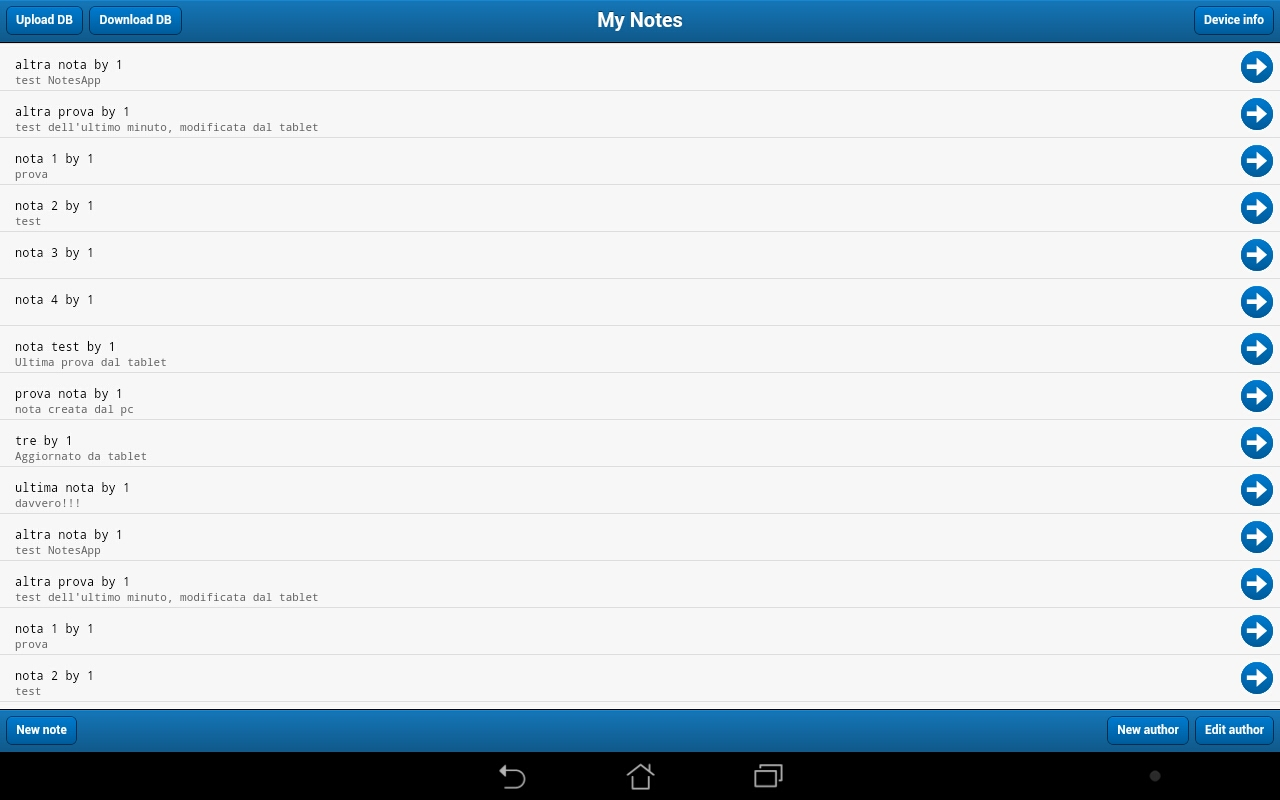
\includegraphics[scale=0.25]{gfx/screenshot/screen_MyNotes}
\caption{Screenshot pagina principale \emph{MyNotes}}
\label{fig:screenshot mynotes}
\end{figure}

\section{SensorDevice}
La realizzazione dell'applicazione \emph{SensorDevice} ha richiesto uno studio approfondito del framework \emph{Apache Cordova} \cite{apache:cordova} e del sistema di plugin che fornisce le interfacce alle funzionalità native dei device mobili.

Per soddisfare i requisiti dell'applicazione sono stati utilizzati i seguenti plugin:
\begin{description}
\item[Barcode\footnotemark:]\footnotetext{Plugin di terze parti \cite{wildabeast:barcodeScanner} trovato nella raccolta presente nel sito di \emph{PhoneGap}.} permette di leggere un barcode tramite la fotocamera del dispositivo;
\item[Camera:] permette di catturare un'immagine tramite la fotocamera o la galleria del dispositivo;
\item[Capture:] permette di catturare file audio, video e immagini tramite la fotocamera e il microfono del dispositivo ;
\item[Connection:] permette di testare la connettività del dispositivo e di recuperarne la tipologia;
\item[Contacts:] permette di consultare e modificare la rubrica del dispositivo;
\item[Device:] permette di visualizzare le informazioni proprie del dispositivo;
\item[File:] permette di scrivere o leggere un file nella memoria del dispositivo;
\item [Geolocation]: permette di visualizzare la posizione corrente del dispositivo;
\end{description}

\clearpage

\subsection{Sviluppo interfaccia grafica}

\begin{figure}[htb]
\centering
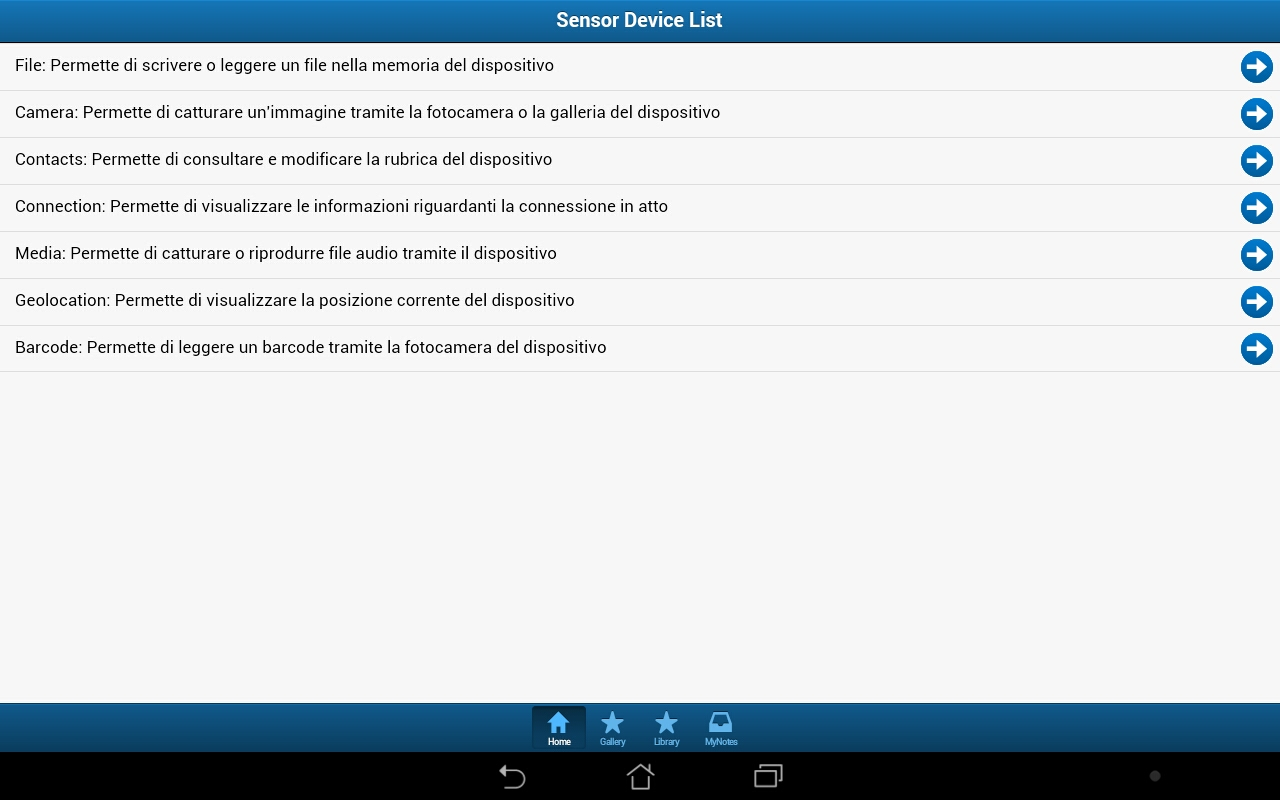
\includegraphics[scale=0.25]{gfx/screenshot/screen_sensorDevice}
\caption{Screenshot pagina principale \emph{SensorDevice}}
\label{fig:screenshot sensordevice}
\end{figure}

Lo sviluppo della \ac{GUI} ha prodotto il risultato visibile in figura \ref{fig:screenshot sensordevice}, dove si vede la lista di funzionalità utilizzabili dall'utente e in basso la barra di navigazione con le pagine disponibili.

L'interfaccia è volutamente molto semplice in quanto l'aspetto grafico non era tra gli obiettivi dello stage; la sua funzione, infatti, è solamente quella di illustrare all'utente le potenzialità offerte e permettergli di selezionarle.

La pagina che ha richiesto un lavoro più accurato è stata la form di compilazione delle informazioni personali dell'utente che viene utilizzata per realizzare il salvataggio dei dati nella memoria fisica del dispositivo; l'immagine è disponibile in figura \ref{fig:screenshot file sensordevice}.

\begin{figure}[htb]
\centering
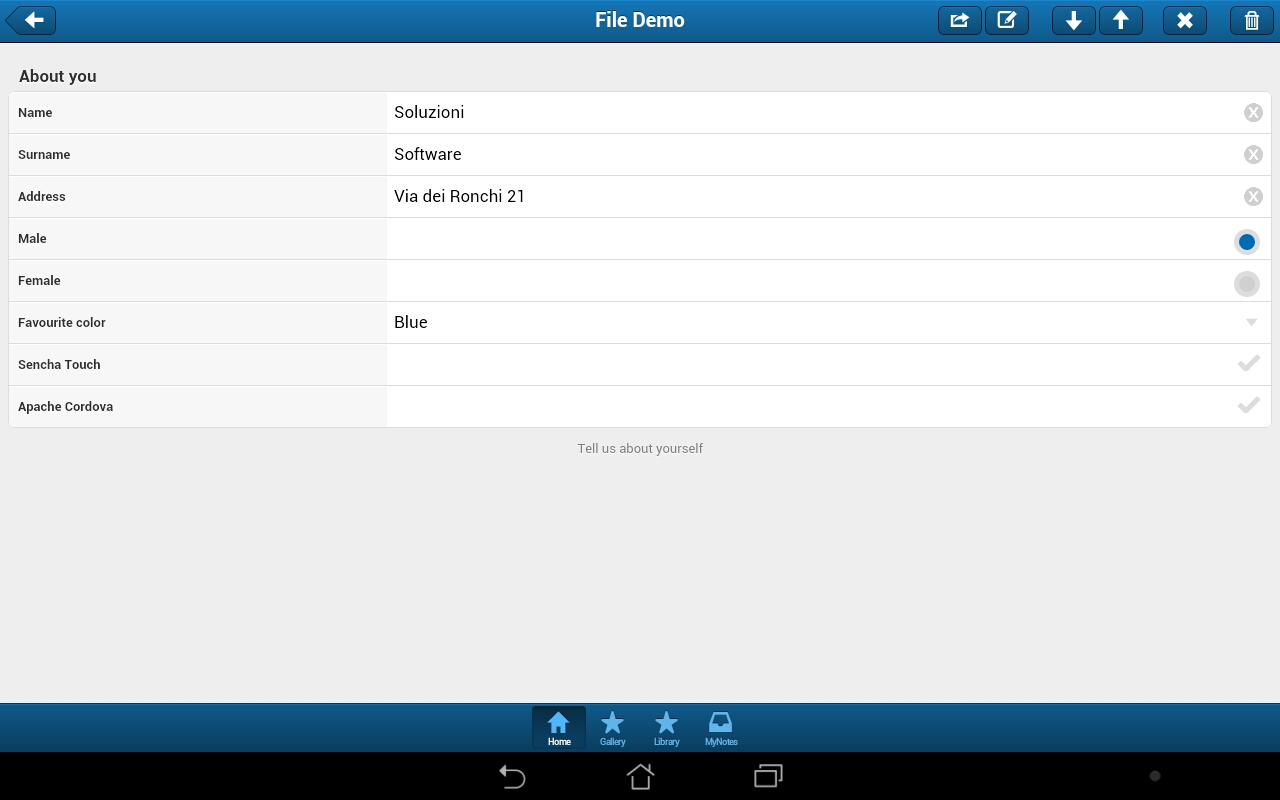
\includegraphics[scale=0.25]{gfx/screenshot/screen_file_sensorDevice}
\caption{Screenshot form informazioni personali \emph{SensorDevice}}
\label{fig:screenshot file sensordevice}
\end{figure}

\subsection{Utilizzo plugin Apache Cordova}
Il vantaggio nell'utilizzo di \emph{Cordova} risiede nella disponibilità di numerosi plugin che forniscono interfacce per le più comuni periferiche e funzionalità native dei device in commercio.

Grazie a tale caratteristica è stato semplice utilizzare le \ac{API} del framework per sviluppare i componenti previsti; la documentazione si è rivelata precisa ed affidabile e il tool a riga di comando ha completato con successo ogni tentativo di compilazione.

\subsection{Integrazione MyNotes}
L'ultimo passo per rendere completa l'applicazione è stato quello di integrare l'applicazione \emph{MyNotes} in una pagina di \emph{SensorDevice} in modo da fornire all'azienda una sola applicazione contenente tutto il lavoro svolto e che rendesse visibili tutte le funzionalità utilizzabili con l'utilizzo congiunto dei due framework utilizzati.

In figura \ref{fig:screenshot mynotes sensordevice} si può vedere la pagina relativa a \emph{MyNotes} all'interno di \emph{SensorDevice}; l'applicazione ha subito un naturale restyling dovuto alla diversa struttura grafica delle pagine ed è stata aggiunta la possibilità di salvare le note presenti sulla memoria del dispositivo.

\begin{figure}[htb]
\centering
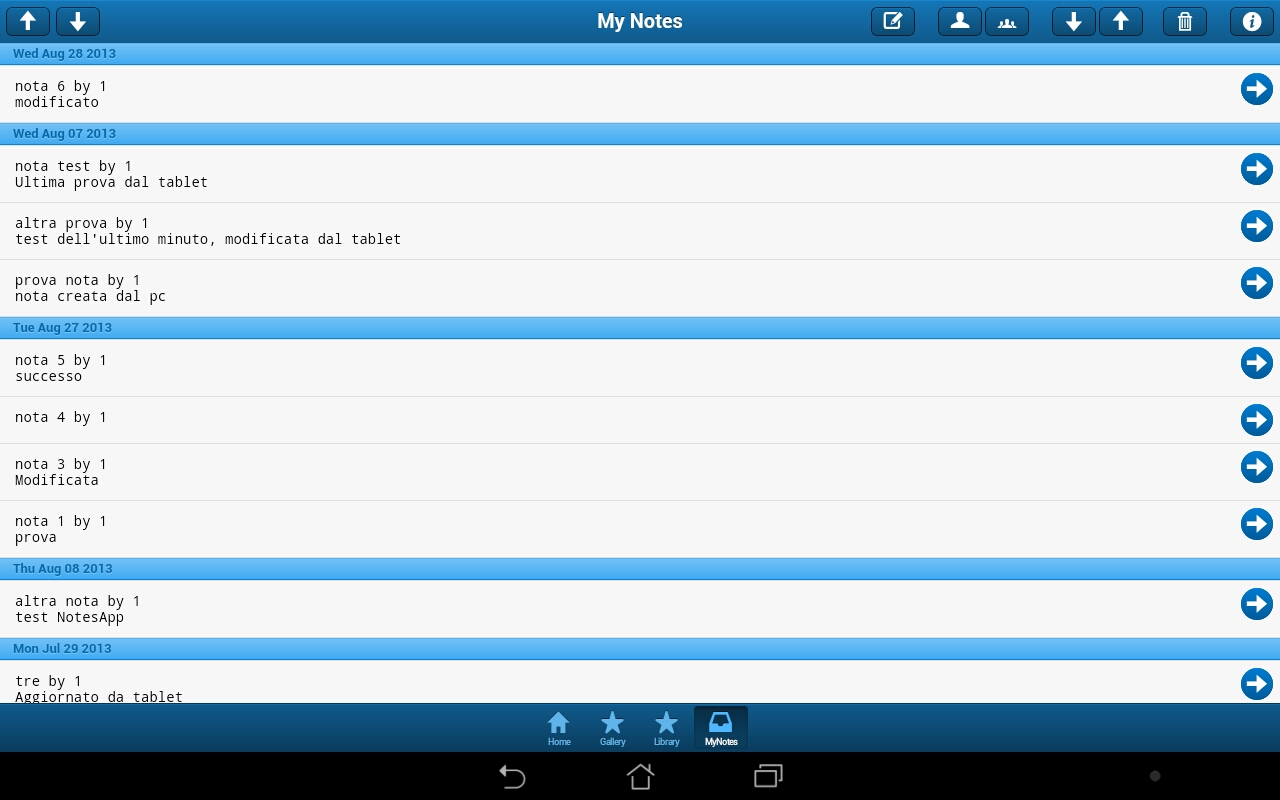
\includegraphics[scale=0.25]{gfx/screenshot/screen_sensor_myNotes}
\caption{Screenshot pagina \emph{MyNotes} integrata in \emph{SensorDevice}}
\label{fig:screenshot mynotes sensordevice}
\end{figure}

\section{ArchitectApp}
Con l'uscita di \emph{Sencha Touch 2.3} \cite{sencha:touch23} e dopo aver concluso positivamente i due prototipi, è stato effettuato uno studio sulle nuove caratteristiche offerte dal nuovo framework: in esso infatti sono stati aggiunte delle classi \emph{wrapper} alle \ac{API} di \emph{Cordova} rendendo ancora più semplice il lavoro dello sviluppatore.

Inoltre, è stato migliorato il tool di compilazione \emph{Sencha Cmd} che automaticamente richiama \emph{Cordova \ac{CLI}} per effettuare la build del sistema creando i file necessari per l'installazione sui dispositivi mobili.

Per provare questa nuova versione si è deciso di utilizzare \emph{Sencha Architect} \cite{sencha:architect}, strumento \emph{drag-and-drop} per la creazione di interfacce grafiche e di sfruttare l'incremento di velocità nello sviluppo per realizzare una nuova versione di \emph{SensorDevice}.

Si è iniziato a creare un'interfaccia ad hoc per tablet, divisa in due zone, una riservata al menu e l'altra studiata per ospitare i componenti utilizzati per visualizzare le funzionalità presenti all'utente.

Grazie a tale editor grafico è stato molto semplice creare una \ac{GUI} più complessa e articolata rispetto a quanto eseguito su editor testuale, evidenziando i pregi delle componenti grafiche del framework e sopperendo alle mancanze della documentazione spesso risulta essere molto enigmatica.

Il prodotto di questa attività è visibile in figura \ref{fig:screenshot device architect}, dove si può vedere la pagina che visualizza le informazioni proprie del dispositivo in uso ricavate con il relativo plugin di \emph{Apache Cordova}.

\begin{figure}[htb]
\centering
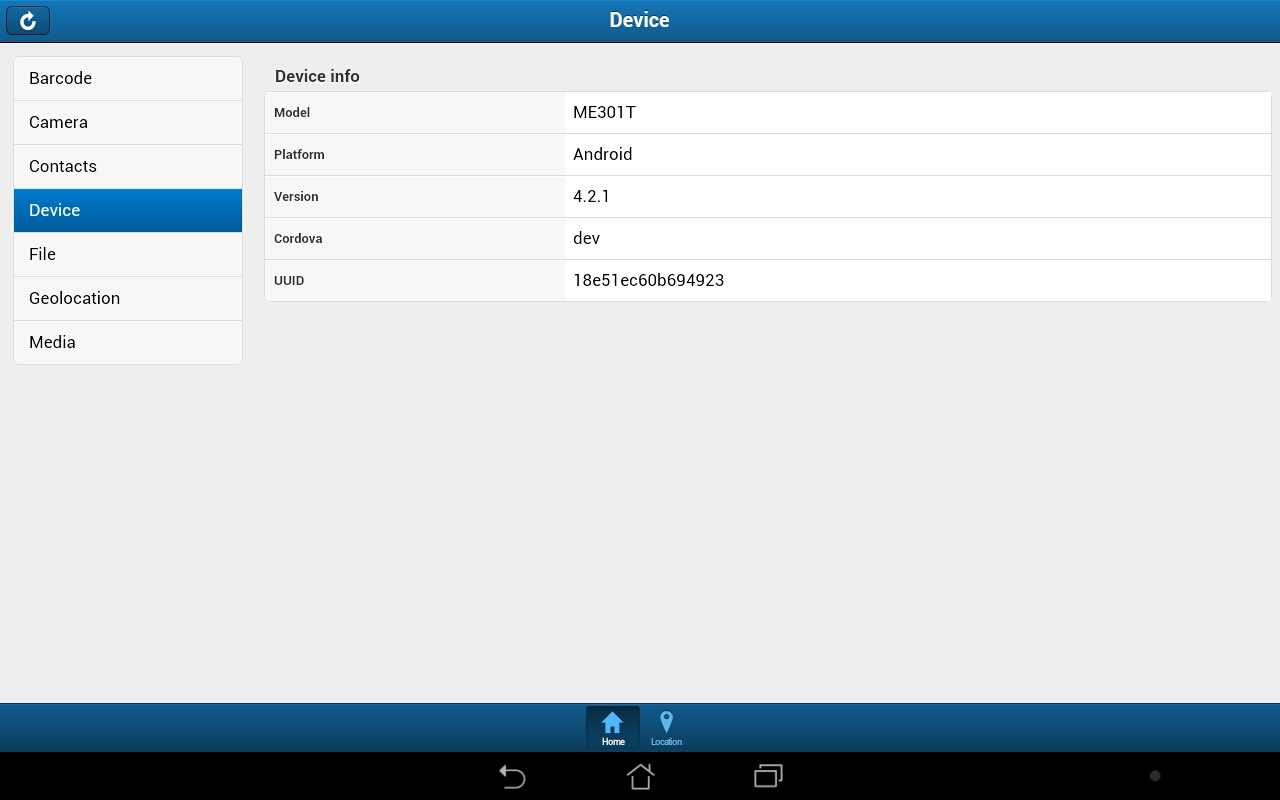
\includegraphics[scale=0.25]{gfx/screenshot/screen_device_architect}
\caption{Screenshot pagina informazioni device \emph{ArchitectApp}}
\label{fig:screenshot device architect}
\end{figure}
%************************************************
\chapter{Test}\label{ch:test}
%************************************************
Il seguente capitolo descrive i test funzionali che sono stati svolti sui prototipi per verificarne il corretto funzionamento e la corrispondenza con i casi d'uso e i requisiti emersi dall'analisi effettuata.

Tali test sono stati eseguiti numerose volte e si sono svolti mantenendo collegato il dispositivo al notebook mediante cavo USB con lo scopo di sfruttare la console di debug fornita da \emph{Eclipse} per monitorare il funzionamento dei prototipi.
Infatti ad ogni metodo presente nei prototipi degli oggetti sviluppati è stato inserito almeno un comando di output a console per identificare il flusso del programma.
Questa tecnica ha consentito di individuare alcuni malfunzionamenti e di comprendere meglio gli oggetti ritornati da alcune chiamate di metodi propri dei framework utilizzati, i quali erano documentati in modo carente o erroneo.

I test svolti presentano un codice identificativo composto dal prefisso \emph{T} seguito da un codice numerico progressivo.

\section{MyNotes}
\subsection{T1 - Visualizzazione note}
\begin{description}
\item[descrizione]: Dopo aver avviato con successo l'applicazione, l'utente deve vedere una lista delle note esistenti; nel caso che l'applicazione venga avviata per la prima volta, la lista deve risultare vuota.
\item[requisito verificato]: R0F1, R0F1.1
\item[esito]: \emph{superato}
\end{description}

\subsection{T2 - Creazione nuova nota}
\begin{description}
\item[descrizione]: \hfill
	\begin{enumerate}
	\item L'utente seleziona la creazione di una nuova nota e il sistema visualizza la pagina di compilazione;
	\item L'utente compila i campi relativi alla nuova nota;
	\item L'utente sceglie di salvare la nota e il sistema la salva correttamente e la visualizza nella lista;
	\end{enumerate}
\item[requisiti verificati]: R0F1, R0F1.2, R0F1.2.1, R0F1.2.2
\item[esito]: \emph{superato}
\end{description}

\subsection{T3 - Eliminazione nuova nota}
\begin{description}
\item[descrizione]: \hfill
	\begin{enumerate}
	\item L'utente seleziona la creazione di una nuova nota e il sistema visualizza la pagina di compilazione;
	\item L'utente compila i campi relativi alla nuova nota;
	\item L'utente sceglie di eliminare la nuova nota e il sistema chiede conferma di eliminazione;
	\item L'utente conferma la cancellazione della nota e il sistema elimina la nuova nota;
	\end{enumerate}
\item[requisiti verificati]: R0F1, R0F1.2, R0F1.2.1, R0F1.2.3, R0F1.2.4, R0F1.2.4.1
\item[esito]: \emph{superato}
\end{description}

\subsection{T4 - Annullamento eliminazione nuova nota}
\begin{description}
\item[descrizione]: \hfill
	\begin{enumerate}
	\item L'utente seleziona la creazione di una nuova nota e il sistema visualizza la pagina di compilazione;
	\item L'utente compila i campi relativi alla nuova nota;
	\item L'utente sceglie di eliminare la nuova nota e il sistema chiede conferma di eliminazione;
	\item L'utente annulla la cancellazione della nota e il sistema annulla l'eliminazione;
	\end{enumerate}
\item[requisiti verificati]: R0F1, R0F1.2, R0F1.2.1, R0F1.2.3, R0F1.2.4, R0F1.2.4.2
\item[esito]: \emph{superato}
\end{description}

\subsection{T5 - Modifica nota esistente}
\begin{description}
\item[descrizione]: \hfill
	\begin{enumerate}
	\item L'utente seleziona una nota esistente dalla lista e il sistema visualizza la pagina di modifica;
	\item L'utente effettua le modifiche desiderate;
	\item L'utente sceglie di salvare le modifiche apportate alla nota e il sistema la salva correttamente e la visualizza nella lista;
	\end{enumerate}
\item[requisiti verificati]: R0F1, R0F1.3, R0F1.3.1, R0F1.3.2
\item[esito]: \emph{superato}
\end{description}

\subsection{T6 - Eliminazione nota esistente}
\begin{description}
\item[descrizione]: \hfill
	\begin{enumerate}
	\item L'utente seleziona una nota esistente dalla lista e il sistema visualizza la pagina di modifica;
	\item L'utente sceglie di eliminare la nota e il sistema chiede conferma di eliminazione;
	\item L'utente conferma la cancellazione della nota e il sistema elimina la nota esistente;
	\end{enumerate}
\item[requisiti verificati]: R0F1, R0F1.3, R0F1.3.3, R0F1.3.4, R0F1.3.4.1
\item[esito]: \emph{superato}
\end{description}

\subsection{T7 - Annullamento eliminazione nota esistente}
\begin{description}
\item[descrizione]: \hfill
	\begin{enumerate}
	\item L'utente seleziona la creazione di una nota esistente e il sistema visualizza la pagina di modifica;
	\item L'utente sceglie di eliminare la nota e il sistema chiede conferma di eliminazione;
	\item L'utente annulla la cancellazione della nota e il sistema annulla l'eliminazione;
	\end{enumerate}
\item[requisiti verificati]: R0F1, R0F1.3, R0F1.3.3, R0F1.3.4, R0F1.3.4.2
\item[esito]: \emph{superato}
\end{description}

\subsection{T8 - Visualizzazione autori}
\begin{description}
\item[descrizione]: Dopo aver avviato con successo l'applicazione, l'utente deve visualizzare la lista degli autori esistenti; nel caso sia il primo avvio dell'applicazione o che non siano stati ancora creati degli autori, la lista deve risultare vuota.
\item[requisiti verificati]: R0F2, R0F2.1
\item[esito]: \emph{superato}
\end{description}

\subsection{T9 - Creazione nuovo autore}
\begin{description}
\item[descrizione]: \hfill
	\begin{enumerate}
	\item L'utente seleziona la creazione di un nuovo autore e il sistema visualizza la pagina di compilazione;
	\item L'utente compila i campi relativi alla nuovo autore;
	\item L'utente sceglie di salvare l'autore e il sistema lo salva correttamente e lo visualizza nella lista;
	\end{enumerate}
\item[requisiti verificati]: R0F2, R0F2.2, R0F2.2.1, R0F2.2.2
\item[esito]: \emph{superato}
\end{description}

\subsection{T10 - Eliminazione nuovo autore}
\begin{description}
\item[descrizione]: \hfill
	\begin{enumerate}
	\item L'utente seleziona la creazione di un nuova autore e il sistema visualizza la pagina di compilazione;
	\item L'utente compila i campi relativi al nuovo autore;
	\item L'utente sceglie di eliminare il nuovo autore e il sistema chiede conferma di eliminazione;
	\item L'utente conferma la cancellazione dell'autore e il sistema elimina il nuovo autore;
	\end{enumerate}
\item[requisiti verificati]: R0F2, R0F2.2, R0F2.2.1, R0F2.2.3, R0F2.2.4, R0F2.2.4.1
\item[esito]: \emph{superato}
\end{description}

\subsection{T11 - Annullamento eliminazione nuovo autore}
\begin{description}
\item[descrizione]: \hfill
	\begin{enumerate}
	\item L'utente seleziona la creazione di un nuovo autore e il sistema visualizza la pagina di compilazione;
	\item L'utente compila i campi relativi al nuovo autore;
	\item L'utente sceglie di eliminare il nuovo autore e il sistema chiede conferma di eliminazione;
	\item L'utente annulla la cancellazione dell'autore e il sistema annulla l'eliminazione;
	\end{enumerate}
\item[requisiti verificati]: R0F2, R0F2.2, R0F2.2.1, R0F2.2.3, R0F2.2.4, R0F2.2.4.2
\item[esito]: \emph{superato}
\end{description}

\subsection{T12 - Modifica autore esistente}
\begin{description}
\item[descrizione]: \hfill
	\begin{enumerate}
	\item L'utente seleziona un autore esistente dalla lista e il sistema visualizza la pagina di modifica;
	\item L'utente effettua le modifiche desiderate;
	\item L'utente sceglie di salvare le modifiche apportate all'autore e il sistema lo salva correttamente e lo visualizza nella lista;
	\end{enumerate}
\item[requisiti verificati]: R0F2, R0F2.3, R0F2.3.1, R0F2.3.2
\item[esito]: \emph{superato}
\end{description}

\subsection{T13 - Eliminazione autore esistente}
\begin{description}
\item[descrizione]: \hfill
	\begin{enumerate}
	\item L'utente seleziona un autore esistente dalla lista e il sistema visualizza la pagina di modifica;
	\item L'utente sceglie di eliminare l'autore e il sistema chiede conferma di eliminazione;
	\item L'utente conferma la cancellazione dell'autore e il sistema elimina l'autore esistente;
	\end{enumerate}
\item[requisiti verificati]: R0F2, R0F2.3, R0F2.3.3, R0F2.3.4, R0F2.3.4.1
\item[esito]: \emph{superato}
\end{description}

\subsection{T14 - Annullamento eliminazione autore esistente}
\begin{description}
\item[descrizione]: \hfill
	\begin{enumerate}
	\item L'utente seleziona la creazione di un autore esistente e il sistema visualizza la pagina di modifica;
	\item L'utente sceglie di eliminare l'autore e il sistema chiede conferma di eliminazione;
	\item L'utente annulla la cancellazione dell'autore e il sistema annulla l'eliminazione;
	\end{enumerate}
\item[requisiti verificati]: R0F2, R0F2.3, R0F2.3.3, R0F2.3.4, R0F2.3.4.2
\item[esito]: \emph{superato}
\end{description}

\subsection{T15 - Download dati dal server}
\begin{description}
\item[descrizione]: Dopo aver avviato con successo l'applicazione, l'utente decide di effettuare il download dei dati presenti nel server; il sistema si collega al server, scarica i dati e li unisce con quelli presenti nel dispositivo.
Nel caso non siano presenti dati nel server, l'utente non nota nessuna modifica alla lista delle note e degli autori.
\item[requisiti verificati]: R0F3, R0F3.1
\item[esito]: \emph{superato}
\end{description}

\subsection{T16 - Upload dati sul server}
\begin{description}
\item[descrizione]: Dopo aver avviato con successo l'applicazione, l'utente decide di effettuare l'upload sul server dei dati presenti nel dispositivo; il sistema prepara i dati e li spedisce al server.
Nel caso non siano presenti dati nel dispositivo, il sistema invia un pacchetto vuoto.
\item[requisiti verificati]: R0F3, R0F3.2
\item[esito]: \emph{superato}
\end{description}

\subsection{T17 - Gestione informazioni del dispositivo}
\begin{description}
\item[descrizione]: \hfill
	\begin{itemize}
	\item Dopo aver avviato con successo l'applicazione, l'utente decide di compilare le informazioni del dispositivo, inserendo un nome per il device e una descrizione;
	\item L'utente sceglie di salvare le informazioni immesse e il sistema le salva correttamente.
	\end{itemize}
\item[requisiti verificati]: R0F4, R0F4.1, R0F4.2
\item[esito]: \emph{superato}
\end{description}

\subsection{Tracciamento requisiti - test}
Di seguito viene riportata la tabella che traccia i singoli requisti dell'applicazione ai test effettuati che li soddisfano.
%**************************************
%    tabella tracciamento requisiti test MyNotes
%**************************************
\rowcolors{1}{lightCyan}{paleTurquoise}
\begin{longtable}{ll}
\hiderowcolors
\caption{Tracciamento requisiti - test -- MyNotes}
\label{tab:tracciamento requisiti-test mynotes} \\
%intestazione iniziale
\toprule \hiderowcolors
Requisito & Test\\
\midrule
\endfirsthead
%intestazione normale
\hiderowcolors
\multicolumn{2}{l}{\footnotesize\itshape Continua dalla pagina precedente}\\
\toprule \hiderowcolors
Requisito & Test\\
\midrule
\endhead
%piede normale
\midrule \hiderowcolors
\multicolumn{2}{r}{\footnotesize\itshape Continua nella prossima pagina}\\
\endfoot
%piede finale
\bottomrule \hiderowcolors
\multicolumn{2}{r}{\footnotesize\itshape Si conclude dalla pagina precedente}\\
\endlastfoot
%corpo della tabella
\showrowcolors 
R0F1			& T1, T2, T3, T4, T5, T6, T7 \\
R0F1.1			& T1 \\
R0F1.2			& T2, T3, T4 \\
R0F1.2.1		& T2, T3, T4 \\
R0F1.2.2		& T2 \\
R0F1.2.3		& T3, T4 \\
R0F1.2.4		& T3, T4 \\
R0F1.2.4.1		& T3 \\
R0F1.2.4.2		& T4 \\
R0F1.3			& T5, T6, T7 \\
R0F1.3.1		& T5 \\
R0F1.3.2		& T5 \\
R0F1.3.3		& T6, T7 \\
R0F1.3.4		& T6, T7 \\
R0F1.3.4.1		& T6 \\
R0F1.3.4.2		& T7 \\
R0F2			& T8, T9, T10, T11, T12, T13, T14 \\
R0F2.1			& T8 \\
R0F2.2			& T9, T10, T11 \\
R0F2.2.1		& T9, T10, T11 \\
R0F2.2.2		& T9 \\
R0F2.2.3		& T10, T11 \\
R0F2.2.4		& T10, T11 \\
R0F2.2.4.1		& T10 \\
R0F2.2.4.2		& T11 \\
R0F2.3			& T12, T13, T14 \\
R0F2.3.1		& T12 \\
R0F2.3.2		& T12 \\
R0F2.3.3		& T13, T14 \\
R0F2.3.4		& T13, T14 \\
R0F2.3.4.1		& T13 \\
R0F2.3.4.2		& T14 \\
R0F3			& T15, T16 \\
R0F3.1			& T15 \\
R0F3.2			& T16 \\
R0F4			& T17 \\
R0F4.1			& T17 \\
R0F4.2			& T17 \\
\end{longtable}

\section{SensorDevice}
\subsection{T1 - Lettura barcode}
\begin{description}
\item[descrizione]: \hfill
	\begin{itemize}
	\item Dopo aver avviato con successo l'applicazione, l'utente sceglie di effettuare la lettura di un codice a barre;
	\item Il sistema accede alla fotocamera e permette all'utente di inquadrare un codice a barre;
	\item L'utente inquadra il barcode e il sistema lo legge correttamente, chiude la fotocamera, salva il codice letto e lo visualizza.
	\end{itemize}
\item[requisito verificato]: R1F1, R1F9, R1F10
\item[esito]: \emph{superato}
\end{description}

\subsection{T2 - Scatto fotografia}
\begin{description}
\item[descrizione]: \hfill
	\begin{itemize}
	\item Dopo aver avviato con successo l'applicazione, l'utente sceglie di scattare una fotografia;
	\item Il sistema accede alla fotocamera e permette all'utente di scattare una fotografia;
	\item L'utente scatta la fotografia e il sistema chiude la fotocamera e salva l'immagine scattata.
	\end{itemize}
\item[requisito verificato]: R1F2, R1F2.1, R1F2.1.1, R1F10
\item[esito]: \emph{superato}
\end{description}

\subsection{T3 - Recupero immagine da galleria}
\begin{description}
\item[descrizione]: \hfill
	\begin{itemize}
	\item Dopo aver avviato con successo l'applicazione, l'utente sceglie di recuperare un'immagine esistente dalla galleria;
	\item Il sistema accede alla galleria del dispositivo e permette all'utente di selezionare un immagine;
	\item L'utente seleziona l'immagine da importare e il sistema chiude la galleria e salva l'immagine selezionata.
	\end{itemize}
\item[requisito verificato]: R1F2, R1F2.1, R1F2.1.2, R1F10
\item[esito]: \emph{superato}
\end{description}

\subsection{T4 - Cattura video}
\begin{description}
\item[descrizione]: \hfill
	\begin{itemize}
	\item Dopo aver avviato con successo l'applicazione, l'utente sceglie di effettuare la cattura di un video;
	\item Il sistema accede alla fotocamera e permette all'utente di registrare un video;
	\item L'utente realizza un video e il sistema chiude la fotocamera e salva il video realizzato.
	\end{itemize}
\item[requisito verificato]: R1F2, R1F2.2, R1F10
\item[esito]: \emph{superato}
\end{description}

\subsection{T5 - Cattura audio}
\begin{description}
\item[descrizione]: \hfill
	\begin{itemize}
	\item Dopo aver avviato con successo l'applicazione, l'utente sceglie di effettuare la cattura di un file audio;
	\item Il sistema accede al microfono e permette all'utente di registrare una traccia audio;
	\item L'utente registra una traccia audio e il sistema chiude il microfono e salva la traccia realizzata.
	\end{itemize}
\item[requisito verificato]: R1F2, R1F2.3, R1F10
\item[esito]: \emph{superato}
\end{description}

\subsection{T6 - Recupero informazioni dispositivo}
\begin{description}
\item[descrizione]: \hfill
	\begin{itemize}
	\item Dopo aver avviato con successo l'applicazione, l'utente sceglie di recuperare le informazioni proprie del dispositivo;
	\item Il sistema accede al dispositivo e recupera il modello del dispositivo, il sistema operativo installato e la versione, l'\ac{UUID} e la versione di \emph{Cordova} in uso e li visualizza.
	\end{itemize}
\item[requisito verificato]: R1F3, R1F9, R1F10
\item[esito]: \emph{superato}
\end{description}

\subsection{T7 - Recupero posizione corrente}
\begin{description}
\item[descrizione]: \hfill
	\begin{itemize}
	\item Dopo aver avviato con successo l'applicazione, l'utente sceglie di recuperare la posizione corrente tramite il \ac{GPS};
	\item Il sistema accede al ricevitore \ac{GPS} del dispositivo, recupera la posizione corrente, la salva e la visualizza.
	\end{itemize}
\item[requisito verificato]: R1F4, R1F9, R1F10
\item[esito]: \emph{superato}
\end{description}

\subsection{T8 - Recupero contatti rubrica}
\begin{description}
\item[descrizione]: \hfill
	\begin{itemize}
	\item Dopo aver avviato con successo l'applicazione, l'utente sceglie di recuperare i contatti della rubrica presenti nel dispositivo;
	\item Il sistema accede alla rubrica del dispositivo e recupera i contatti presenti, li salva e li visualizza.
	\end{itemize}
\item[requisito verificato]: R1F5, R1F9, R1F10
\item[esito]: \emph{superato}
\end{description}

\subsection{T9 - Salvataggio informazioni personali utente}
\begin{description}
\item[descrizione]: \hfill
	\begin{itemize}
	\item Dopo aver avviato con successo l'applicazione, l'utente sceglie di compilare le informazioni personali accedendo alla pagina dedicata;
	\item L'utente decide di salvare le informazioni immesse e il sistema le salva correttamente.
	\end{itemize}
\item[requisito verificato]: R1F6, R1F6.1, R1F6.2, R1F9, R1F10
\item[esito]: \emph{superato}
\end{description}

\subsection{T10 - Eliminazione informazioni personali utente}
\begin{description}
\item[descrizione]: \hfill
	\begin{itemize}
	\item Dopo aver avviato con successo l'applicazione, l'utente sceglie di eliminare le informazioni personali precedentemente salvate;
	\item Il sistema elimina le informazioni salvate.
	\end{itemize}
\item[requisito verificato]: R1F6, R1F6.3, R1F9, R1F10
\item[esito]: \emph{superato}
\end{description}

\subsection{T11 - Backup informazioni personali utente}
\begin{description}
\item[descrizione]: \hfill
	\begin{itemize}
	\item Dopo aver avviato con successo l'applicazione, l'utente sceglie di effettuare il backup delle informazioni personali salvate sul dispositivo;
	\item Il sistema effettua il salvataggio sulla memoria di massa del dispositivo in un file di testo denominato \code{backupPersonalInfo.txt} e situato nella cartella \code{SensorDevice}.
	\end{itemize}
\item[requisito verificato]: R1F6, R1F6.4
\item[esito]: \emph{superato}
\end{description}

\subsection{T12 - Ripristino informazioni personali utente}
\begin{description}
\item[descrizione]: \hfill
	\begin{itemize}
	\item Dopo aver avviato con successo l'applicazione, l'utente sceglie di effettuare il ripristino delle informazioni personali di cui è stato precedentemente effettuato un backup;
	\item Il sistema recupera le informazioni dal file \code{/sdcard/SensorDevice/backpPersonalInfo.txt} e le salva nello store dedicata sostituendo quelle presenti.
	\end{itemize}
\item[requisito verificato]: R1F6, R1F6.5
\item[esito]: \emph{superato}
\end{description}

\subsection{T13 - Consultazione galleria immagini}
\begin{description}
\item[descrizione]: Dopo aver avviato con successo l'applicazione, l'utente sceglie di consultare la galleria immagini accedendo alla pagina dedicata e il sistema visualizza le immagini presenti; nel caso sia il primo avvio dell'applicazione o non siano presenti immagini la galleria deve risultare vuota.
\item[requisito verificato]: R1F7
\item[esito]: \emph{superato}
\end{description}

\subsection{T14 - Consultazione libreria audio/video}
\begin{description}
\item[descrizione]: Dopo aver avviato con successo l'applicazione, l'utente sceglie di consultare la libreria audio/video accedendo alla pagina dedicata e il sistema visualizza un elenco delle registrazioni audio e video presenti; nel caso sia il primo avvio dell'applicazione o non siano presenti registrazioni la libreria deve risultare vuota.
\item[requisito verificato]: R1F8
\item[esito]: \emph{superato}
\end{description}

\subsection{Tracciamento requisiti - test}
Di seguito viene riportata la tabella che traccia i singoli requisti dell'applicazione ai test effettuati che li soddisfano.
%**************************************
%    tabella tracciamento requisiti test SensorDevice
%**************************************
\rowcolors{1}{lightCyan}{paleTurquoise}
\begin{longtable}{ll}
\hiderowcolors
\caption{Tracciamento requisiti - test -- SensorDevice}
\label{tab:tracciamento requisiti-test sensordevice} \\
%intestazione iniziale
\toprule \hiderowcolors
Requisito & Test\\
\midrule
\endfirsthead
%intestazione normale
\hiderowcolors
\multicolumn{2}{l}{\footnotesize\itshape Continua dalla pagina precedente}\\
\toprule \hiderowcolors
Requisito & Test\\
\midrule
\endhead
%piede normale
\midrule \hiderowcolors
\multicolumn{2}{r}{\footnotesize\itshape Continua nella prossima pagina}\\
\endfoot
%piede finale
\bottomrule \hiderowcolors
%\multicolumn{2}{r}{\footnotesize\itshape Si conclude dalla pagina precedente}\\
\endlastfoot
%corpo della tabella
\showrowcolors 
R1F1			& T1 \\
R1F2			& T2, T3, T4, T5 \\
R1F2.1			& T2, T3 \\
R1F2.1.1		& T2 \\
R1F2.1.2		& T3 \\
R1F2.2			& T4 \\
R1F2.3			& T5 \\
R1F3			& T6 \\
R1F4			& T7 \\
R1F5			& T8 \\
R1F6			& T9, T10, T11, T12 \\
R1F6.1			& T9 \\
R1F6.2			& T9 \\
R1F6.3			& T10 \\
R1F6.4			& T11 \\
R1F6.5			& T12 \\
R1F7			& T13 \\
R1F8			& T14 \\
R1F9			& T1, T6, T7, T8, T9, T10 \\
R1F10			& T1, T2, T3, T4, T5, T6, T7, T8, T9, T10 \\
\end{longtable} 

%************************************************
\chapter{Conclusioni}\label{ch:conclusioni}
%************************************************ 
\section{Risultati}
Il progetto di stage ha prodotto due prototipi che soddisfano tutti i requisiti individuati durante l'attività di analisi; l'azienda era interessata a testare le applicazioni anche su dispositivi basati su \emph{iOS} ma ciò non è stato possibile a causa dei ritardi nell'ottenimento della licenza necessaria per effettuare il processo di build per tale piattaforma.

In particolare è stato possibile integrare efficacemente il modulo \emph{SyncEngine} e testarne il corretto funzionamento all'interno della semplice applicazione \emph{MyNotes} di gestione di note ed autori.

Per quanto riguarda l'applicazione \emph{SensorDevice}, la tabella \ref{tab:funzionalità sensordevice} illustra il comportamento dei framework utilizzati con le funzionalità che l'azienda desiderava testare: l'unica soluzione capace di utilizzare tutte le periferiche presenti in un dispositivo mobile è stata \emph{ApacheCordova}, i cui plugin sono risultati essere di facile utilizzo e di immediata comprensione grazie alla bontà della documentazione.

\begin{table}[htb]
\caption{Resoconto funzionalità testate -- SensorDevice}
\label{tab:funzionalità sensordevice}
\centering
\begin{tabular}{cccc}
\hiderowcolors
\toprule
\multirow{2}*{Funzionalità} & \multicolumn{2}{c}{Sencha Touch} 			& \multirow{2}*{Apache Cordova} \\
\cmidrule(rl) {2-3} 
							& 2.2.1 		& 2.3.0						& \\
\midrule %\showrowcolors
Barcode						& $\circ$ 		& $\circ$					& $\checkmark$ \\
Camera						& $\checkmark$ 	& $\checkmark$				& $\checkmark$ \\
Capture						& $\circ$ 		& $\bullet$					& $\checkmark$ \\
Connection					& $\checkmark$ 	& $\checkmark$				& $\checkmark$ \\
Contacts					& $\bullet$ 	& $\checkmark$				& $\checkmark$ \\
Device						& $\checkmark$ 	& $\checkmark$				& $\checkmark$ \\
File						 	& $\circ$ 		& $\bullet$					& $\checkmark$ \\
Geolocation					& $\checkmark$ 	& $\checkmark$ 				& $\checkmark$ \\					
\bottomrule
\end{tabular}
\begin{quotation}\footnotesize
\item[$\circ$:] non presente
\item[$\bullet$:] presente ma non funzionante
\item[$\checkmark$:] funzionante
\end{quotation}
\end{table}

\emph{Sencha Touch 2} si è rilevato un'ottima soluzione per realizzare l'interfaccia grafica grazie ai numerosi automatismi del framework e all'architettura \ac{MVC} che semplifica la gestione e la separazione delle diverse unità software; purtroppo è risultata essere ancora carente con l'implementazione di un sistema capace di interagire correttamente con i sensori dei device.

La situazione in proposito è migliorata notevolmente con la distribuzione della versione \emph{2.3} del framework ma l'impressione è che il sistema sia ancora immaturo sotto questo punto di vista e con ampi margini di miglioramento.

Un altro aspetto importante da considerare è l'utilizzo di \emph{Sencha Architect} per la realizzazione di una \ac{GUI}: si è rivelato essere uno strumento essenziale per disegnare velocemente ed efficacemente interfacce complesse, fornendo un aiuto indispensabile allo sviluppatore meno esperto.

Nel complesso l'azienda è rimasta soddisfatta del lavoro svolto, sia per i prototipi realizzati sia per la realizzazione della documentazione completa del codice sorgente di \emph{MyNotes} e di \emph{SensorDevice} ma anche del pacchetto \emph{SyncEngine} dando uniformità e continuità agli stage che li hanno prodotti.

\section{Criticità riscontrate}
L'analisi dei requisiti e la progettazione delle applicazioni non hanno generato problemi rilevanti, sia per la natura esplorativa dello stage sia per il supporto ricevuto dal tutor aziendale.

Le difficoltà maggiori si sono avute nella corretta interpretazione della documentazione \emph{Sencha} che in molti punti si è rivelata essere molto carente e imprecisa, lasciando ai commenti degli utilizzatori il compito di chiarire dubbi e inesattezze.

Anche la consultazione del forum ufficiale spesso è risultata vana in quanto, davanti alla richieste d'aiuto, gli sviluppatori e i progettisti \emph{Sencha} non sempre riescono a dare soluzioni efficaci, lasciando in sospeso le conversazioni o dando risposte molto vaghe e poco utili nella pratica.

Un'ulteriore problema si è avuto con l'integrazione dei due framework: le guide trovate in internet sono state utili per capire il singolo funzionamento dei framework ma, facendo riferimento a vecchie versioni degli stessi e risultando in alcuni casi anche in contrasto tra loro, sono state poco utili per la soluzione al problema: sono serviti diversi tentativi per comprendere la corretta tecnica.
Solamente l'arrivo di \emph{Sencha Touch 2.3} ha risolto parzialmente il problema creando degli \emph{adapter} verso le \ac{API} di \emph{Apache Cordova}, anche se alcuni di questi, come \emph{Device Capture} e \emph{Device File} presentano dei bug che al tempo dello stage non erano risolti.

\section{Conoscenze acquisite}
L'attività di stage mi ha dato la possibilità di vivere una realtà lavorativa in un'azienda solida, seguito da personale qualificato, facendomi mettere in pratica, anche se solo per un breve periodo, le conoscenze che ho acquisito attraverso gli studi universitari e dandomi la possibilità di approcciare la programmazione per sistemi mobili cogliendone alcuni pregi e difetti.

Mi ha permesso di studiare \emph{Sencha Touch} e \emph{Apache Cordova}: i due framework si sono rivelati essere due strumenti molto interessanti per lo sviluppo di applicazioni mobile multi-piattaforma; se utilizzati insieme infatti danno la possibilità ad uno sviluppatore di realizzare software che sfrutti in modo ottimale i sensori dei device e allo stesso tempo  di donare alle applicazioni un aspetto grafico gradevole e che può essere reso accattivante e personalizzato con poche modifiche.

Infine ho avuto la possibilità di seguire interamente e in prima persona tutte le attività di realizzazione di un prodotto software, dall'analisi iniziale, passando per la progettazione e concludendo con lo sviluppo e i test, dovendo prendere in modo autonomo e responsabile decisioni importanti che mi consentissero di portare a termine con successo il progetto affidatomi.

Mi ritengo quindi molto soddisfatto dell'esperienza vissuta, in parte grazie all'azienda \myCompany che mi ha dato questa possibilità inserendomi in un ambiente stimolante e professionale, ma soprattutto perché mi ha permesso di confrontarmi con le difficoltà di un progetto reale a cui sono riuscito a trovare delle soluzioni efficaci mettendo in pratica le mie capacità.


% ********************************************************************
% Backmatter
%*******************************************************
%\appendix
%\cleardoublepage
%\part{Appendice}

%********************************************************************
% Other Stuff in the Back
%*******************************************************
\cleardoublepage%*******************************************************
% Acronyms
%*******************************************************
%\phantomsection 
\refstepcounter{dummy}
\pdfbookmark[1]{Acronimi}{Acronimi}
\markboth{\spacedlowsmallcaps{Acronimi}}{\spacedlowsmallcaps{Acronimi}}
\chapter*{Acronimi}
\begin{acronym}[UML]
	\acro{PMI}{Piccole e Medie Imprese}
    	
	{\small Le piccole e medie imprese o PMI sono aziende le cui dimensioni rientrano entro certi limiti occupazionali e finanziari prefissati. \par}
    	
	\acro{API}{Application Programming Interface}
	
	
	\acro{UML}{Unified Modeling Language}
	
	
\end{acronym}                      

\cleardoublepage%********************************************************************
% Bibliography
%*******************************************************
% work-around to have small caps also here in the headline
\manualmark
\markboth{\spacedlowsmallcaps{\bibname}}{\spacedlowsmallcaps{\bibname}} % work-around to have small caps also
%\phantomsection 
\refstepcounter{dummy}
\addtocontents{toc}{\protect\vspace{\beforebibskip}} % to have the bib a bit from the rest in the toc
\addcontentsline{toc}{chapter}{\tocEntry{\bibname}}
\bibliographystyle{plainnat}
\label{app:bibliography} 
\bibliography{Bibliography}
%\cleardoublepage\pagestyle{empty}

\hfill

\vfill


\pdfbookmark[0]{Colophon}{colophon}
\section*{Colophon}
This document was typeset using the typographical look-and-feel \texttt{classicthesis} developed by Andr\'e Miede. 
The style was inspired by Robert Bringhurst's seminal book on typography ``\emph{The Elements of Typographic Style}''. 
\texttt{classicthesis} is available for both \LaTeX\ and \mLyX: 
\begin{center}
\url{http://code.google.com/p/classicthesis/}
\end{center}
 
\bigskip

\noindent\finalVersionString

%Hermann Zapf's \emph{Palatino} and \emph{Euler} type faces (Type~1 PostScript fonts \emph{URW
%Palladio L} and \emph{FPL}) are used. The ``typewriter'' text is typeset in \emph{Bera Mono}, 
%originally developed by Bitstream, Inc. as ``Bitstream Vera''. (Type~1 PostScript fonts were made 
%available by Malte Rosenau and
%Ulrich Dirr.)

%\paragraph{note:} The custom size of the textblock was calculated
%using the directions given by Mr. Bringhurst (pages 26--29 and
%175/176). 10~pt Palatino needs  133.21~pt for the string
%``abcdefghijklmnopqrstuvwxyz''. This yields a good line length between
%24--26~pc (288--312~pt). Using a ``\emph{double square textblock}''
%with a 1:2 ratio this results in a textblock of 312:624~pt (which
%includes the headline in this design). A good alternative would be the
%``\emph{golden section textblock}'' with a ratio of 1:1.62, here
%312:505.44~pt. For comparison, \texttt{DIV9} of the \texttt{typearea}
%package results in a line length of 389~pt (32.4~pc), which is by far
%too long. However, this information will only be of interest for
%hardcore pseudo-typographers like me.%
%
%To make your own calculations, use the following commands and look up
%the corresponding lengths in the book:
%\begin{verbatim}
%    \settowidth{\abcd}{abcdefghijklmnopqrstuvwxyz}
%    \the\abcd\ % prints the value of the length
%\end{verbatim}
%Please see the file \texttt{classicthesis.sty} for some precalculated 
%values for Palatino and Minion.
%
%    \settowidth{\abcd}{abcdefghijklmnopqrstuvwxyz}
%    \the\abcd\ % prints the value of the length





%\cleardoublepage%*******************************************************
% Declaration
%*******************************************************
\refstepcounter{dummy}
\pdfbookmark[0]{Declaration}{declaration}
\chapter*{Declaration}
\thispagestyle{empty}
Put your declaration here.
\bigskip
 
\noindent\textit{\myLocation, \myTime}

\smallskip

\begin{flushright}
    \begin{tabular}{m{5cm}}
        \\ \hline
        \centering\myName \\
    \end{tabular}
\end{flushright}

% ********************************************************************
% Game Over: Restore, Restart, or Quit?
%*******************************************************
\end{document}
% ********************************************************************
